\documentclass[aspectratio=169,9pt,dvipsnames]{beamer}
% TODO!: graph combined effects
\usetheme{Boadilla}
\usepackage[utf8]{inputenc}
\usepackage[english]{babel}
\usepackage[T1]{fontenc}

\usepackage{xcolor}
\usepackage{amsmath}
\usepackage{amsfonts}
\usepackage{amssymb}
\usepackage{graphicx}
\usepackage{changepage}
\usepackage{ragged2e}
\usepackage{amsmath,amssymb}
\usepackage{eurosym}
\usepackage{hyperref}
\usepackage{textcomp}
\usepackage[export]{adjustbox}
\usepackage[toc,page]{appendix}
\usepackage{appendixnumberbeamer}
\usepackage{subcaption}

\usepackage{array,multirow,makecell}
\setcellgapes{1pt}
\makegapedcells
\newcolumntype{R}[1]{>{\raggedleft\arraybackslash }b{#1}}
\newcolumntype{L}[1]{>{\raggedright\arraybackslash }b{#1}}
\newcolumntype{C}[1]{>{\centering\arraybackslash }b{#1}}

\newcommand{\compresslist}{%
\setlength{\itemsep}{1pt}%
\setlength{\parskip}{0pt}%
\setlength{\parsep}{0pt}%
}

\beamertemplatenavigationsymbolsempty

\setbeamercolor{structure}{fg=teal}
\setbeamertemplate{itemize item}[circle]
\setbeamertemplate{section in toc}[square]
\setbeamertemplate{subsection in toc}[square]
\setbeamersize{text margin left=1cm, text margin right=1cm}

\usepackage{lmodern}
\usefonttheme[onlymath]{serif}

\definecolor{teal_dark}{RGB}{26,140,140}


% TODO: cite more literature
% check all figures are correctly updated

\justifying

\title[Carbon Tax Aversion]{\huge Yellow Vests, Pessimistic Beliefs, \\ and Carbon Tax Aversion}
\author[Douenne \& \textbf{Fabre}]{American Economic Journal: Economic Policy (forthcoming) \\ $\quad$ \\ \Large Thomas Douenne \& \textbf{Adrien Fabre} \large \\ $\quad$ \\ \textit{UvA (Amsterdam) \quad \textbf{ETH (Zürich)}}}
\date[\insertsection]{Hertie School -- January 13, 2022}


\begin{document}

	\begin{frame}

\titlepage
%\thispagestyle{empty}

	\end{frame}

\AtBeginSection[]
{
  \begin{frame}
  \tableofcontents[currentsection]
  \end{frame} 
}

    \begin{frame}{Are French people ecologist?}%\addtocounter{framenumber}{-1}

\begin{figure}[h!]
\centering
\includegraphics[width=.74\textwidth]{Images/GJ.jpg}
\caption{Some Yellow Vests}
\end{figure}
% Twice as more are preoccupied by environment (86%) than by insecurity (DREES, 2019) https://drees.solidarites-sante.gouv.fr/IMG/pdf/dd35.pdf
% Majority gives priority to environment rather than employment or growth (50% vs. 34%) (Gougou, Persico, 2019 https://www.lemonde.fr/idees/article/2019/04/25/la-cohesion-de-la-societe-francaise-n-est-pas-aussi-menacee-qu-on-le-croit_5454574_3232.html)

% The big obstacle to the carbon tax is social acceptance. We've seen this with the Yellow Vests movement as the increase in the carbon tax was the motive for its first protest in november 2018.  At the same time, recent survey shows that 90% of French are preoccupied by CC (twice as more as insecurity). What can explain this seemingly paradoxical attitude towards carbon tax? A simple hypothesis is that people oppose the carbon tax because it is regressive. And if the revenues of the tax were redistributed equally among households, we call this a Tax & Dividend policy, then people would support it because it would be fair and most people would benefit from it financially. But is it really sufficient? For that, you need that people hold beliefs that correspond to the properties of the tax, you need to know that it's progressive for example. We address this question based on a new large survey of the French population, conducted in the middle of the YV crisis (Feb/Mar 2019). To give you a primer of the results, most people oppose the T&D...

% As you know, it's the increase in carbon tax that triggered the social unrest of the yellow vests, as it was the motive for its first protest in november 2018. At the same time, recent survey shows that 90% of French are preoccupied by CC (twice as more as insecurity). We conduct a survey to understand this seemingly paradoxical attitude towards carbon tax. In particular, we want to test whether a Tax & Dividend reform, i.e. a carbon tax with desirable distributive properties, would generate enough support. Our design allows to distinguish pure preferences effects from beliefs over the properties of the tax. Indeed, three beliefs are key to accept the tax: believing that the reform is in one's own interest, that it's effective and that it's socially fair, i.e. progressive. We measure to what extent people share these beliefs, how potential biases in these beliefs are affected when new info is provided, and we quantify the effects that these motivating beliefs have on the acceptance of the tax.
    \end{frame}
    
%      \begin{frame}{Relation to literature}
     
% % \begin{itemize}
% %     \item Surveys on the topic: Carattini et al. (2018), Klenert et al. (2018)
%     % \item Altruistic vs. egoistic motives / beliefs vs. values: Stern et al. (1993)
%     % \item Correlation between carbon tax acceptance and self-interest: Thalmann (2004)
%     % \item Higher approval when distributional issues addressed: Bristow et al. (2010), Brannlund \& Persson (2012)
%     % \item Belief that tax is ineffective: Baranzini \& Carattini (2017), Dresner et al. (2006)
%     % \item Effectiveness and distributional effects matter more than self-interest: Kallbekken \& Sælen (2011)
% % \end{itemize}

% Surveys on the topic: Carattini et al. (2018), Klenert et al. (2018).

% \medskip

% Three main determinants of carbon tax acceptance: self-interest, fairness and environmental effectiveness.

% \medskip

% \textbf{Our contribution:} run a survey to:
% \begin{enumerate}
%     \item test previous results on a representative sample of the French population;
%     \item disentangle erroneous beliefs from \textit{pure} effects of preferences;
%     \item quantify biases regarding the costs of carbon tax;
%     \item show persistence of beliefs over carbon tax;
%     \item estimate causal effects.
% \end{enumerate}

%     \end{frame}

    \begin{frame}{Motivations}

How to avoid regressivity of carbon tax? \vspace{1cm}

$\rightarrow$ \textbf{Tax \& Dividend}: redistributing equally the revenues. Makes it:

\vspace{0.3cm}

\begin{itemize}
    \item progressive \textcolor{teal_dark}{{\small \textit{(e.g. West \& Williams, 2004; Bento et al., 2009; Williams et al., 2015; Douenne, 2020)}}}.
    
    \vspace{0.25cm}
    
    \item supported by 3,354 economists in \textcolor{teal_dark}{{\small \textit{The Wall Street Journal (2019)}}}, "To maximize the fairness and political viability of a rising carbon tax".
\end{itemize}

\vspace{0.4cm}
\pause

\textit{With a design ensuring desirable properties, a policy should be supported.}

\vspace{0.35cm}

\textbf{But is it really sufficient?}

    \end{frame}
    \begin{frame}{This paper}

Based on a large survey representative of the French population, we show that:

\vspace{0.3cm}

\begin{enumerate}[<+->]
    \item Most people oppose a Tax \& Dividend \vspace{0.3cm}
    
    \item They hold pessimistic beliefs about it
    \begin{itemize}
    	\item e.g. 70\% expected to win, only 14\% think they would
    \end{itemize} \vspace{0.15cm}
    
    \item These beliefs may be partially formed through distrust and/or motivated reasoning \vspace{0.3cm}
    
    \item Rejection is driven by pessimistic beliefs: convincing people of the true incidence and environmental effectiveness would suffice to generate large majority approval
\end{enumerate}

\pause 
\vspace{0.5cm}

$\rightarrow$ \textit{Example of a welfare-improving policy rejected due to pessimistic beliefs.}

    \end{frame}
    \begin{frame}{Contributions}

\begin{itemize}
    \item \textbf{Political economy of the carbon tax:}

    \vspace{0.2cm}

    Three key motives for acceptance: \\ \textcolor{teal_dark}{\textit{{\small (See review by Carattini et al. (2018) or synthesis by Klenert et al. (2018))}}} 
    \begin{itemize}
    \item self-interest \textcolor{teal_dark}{{\small \textit{(Thalmann, 2004)}}}
    \item environmental effectiveness \textcolor{teal_dark}{{\small \textit{(Bristow et al 2010; Brannlund \& Persson 2012)}}}
    \item progressivity \textcolor{teal_dark}{{\small \textit{(Kallbekken \& Sælen, 2011; Baranzini \& Carattini, 2017)}}} %Maestre-Andrés
    \end{itemize}
    \vspace{0.3cm}
    
% Oral:    But two main shortcomings: 1) do not disentangle beliefs from preferences; 2) rely on correlations between proxies of beliefs and approval to identify effects of preferences.
    
    %\pause
    %\vspace{0.4cm}
    \pause
    $\rightarrow$ We are the first to: \vspace{0.15cm}
    \begin{enumerate}[<+->]
        \item Estimate objective net gain from the reform\vspace{0.15cm}
        \item Acknowledge and quantify biases in perceptions \vspace{0.15cm}
        \item Estimate causal effects of motives on acceptance
    \end{enumerate}

	\vspace{0.6cm}    
    \pause 
    \item \textbf{Beliefs formation:} \vspace{0.2cm}
    \begin{enumerate}[<+->]
        \item Add new evidence on link between beliefs and preferences for policies \textcolor{teal_dark}{{\small \textit{(e.g. Alesina \& Angeletos, 2005; Bénabou \& Tirole, 2006; Alesina et al., 2018)}}} \vspace{0.15cm}     
        \item Bi-directional causality through directional motivated reasoning \textcolor{teal_dark}{{\small \textit{(e.g. Kunda, 1990; Kahan, 2013; Bénabou \& Tirole, 2016; Druckman \& McGrath, 2019; Little, 2019)}}}
\end{enumerate}
\end{itemize}


% Fill more specific references

    \end{frame}
\section{Survey and data}

%     \begin{frame}{Survey data collection}

% \begin{itemize}
%     \item 3002 responses collected on-line in February/March 2019
%     \item Representative along: gender, age, education, profession, size of town, region
%     %\item Median duration: 19 min, important questions in the first half
%     %\item We exclude: 4\% of respondents answering in less than 7 min, 9\% who fail test of quality
%     %\item We flag 273 inconsistent answers, such as too high fuel economy or incomes: they are not correlated with our main variables of interest
% \end{itemize} %\beamergotobutton{\href{https://hbs.qualtrics.com/jfe/form/SV_9zqdJWZXgpWfjsF}{See the questionnaire}}
%     \hspace{0.5cm}
% 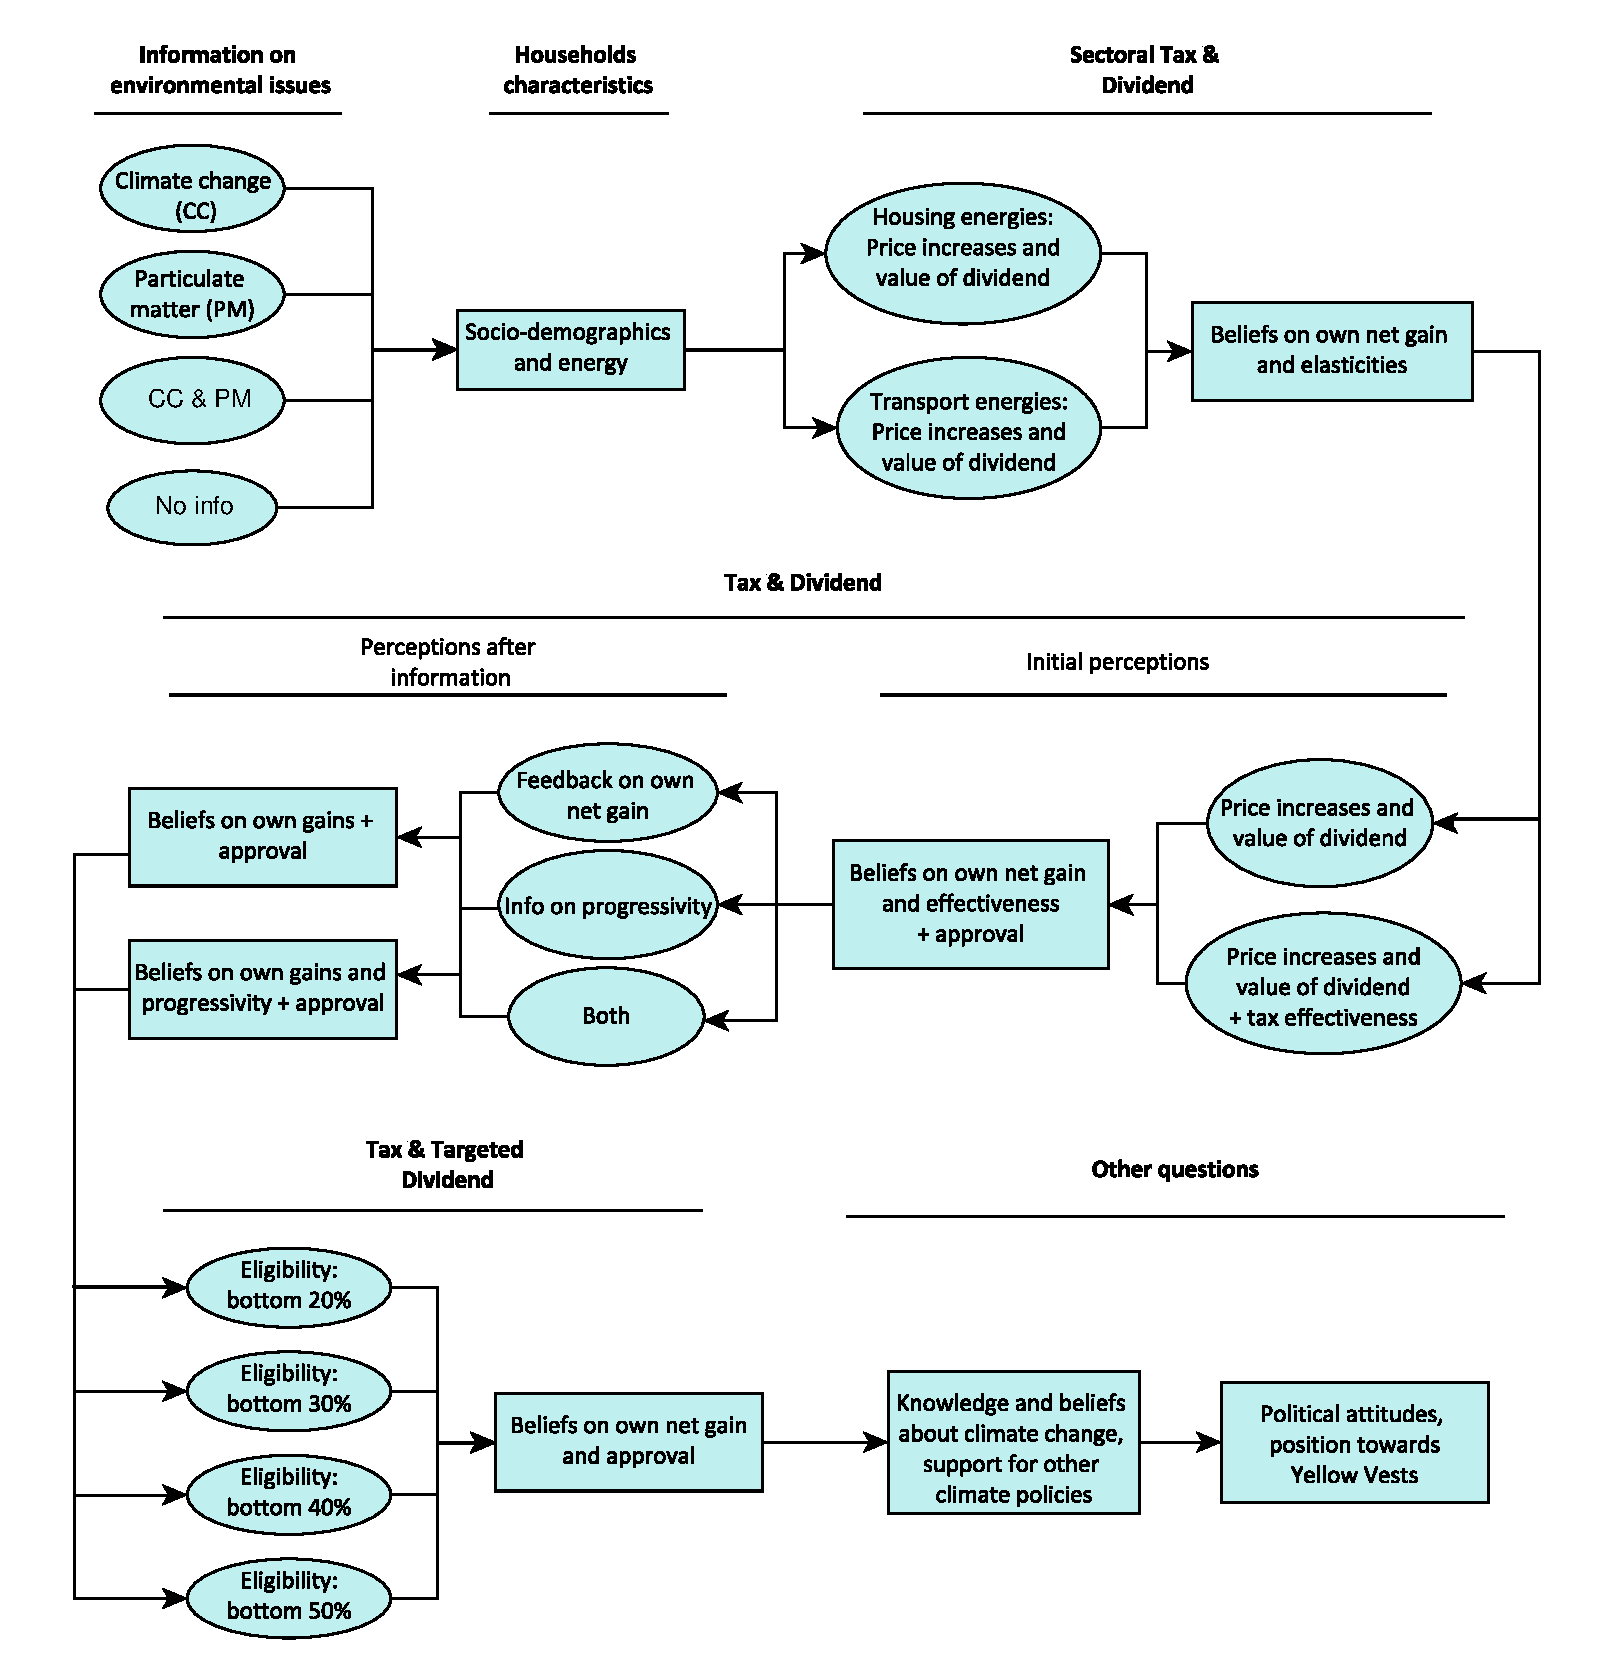
\includegraphics[scale=0.45,left]{Images/diagram_survey.png}

%     \end{frame}

     
    

%     \begin{frame}{French households surveys}
%     \label{insee}
% \begin{itemize}
%     \item We estimate net gains of respondents using another Insee survey: 
%     \begin{itemize}
%         \item \textit{Enquête Logement 2013} (EL): 27,000 HH, good on housing
%         \item increase in housing expenditures = $\beta_0$ + $\beta_f$ fuel + $\beta_g$ gas + $\beta_s$ surface \hyperlink{reg_housing}{\beamergotobutton{See regressions}}
%         \item increase in transport energy expenditures computed directly from HH characteristics
%     \end{itemize}
%     \item We estimate the revenues of the reform with the database of Douenne (2018) that matches two Insee surveys:
%     \begin{itemize}
%         \item \textit{Budget de Famille 2011} (BdF): 10,000 HH, good on housing, not on transport
%         \item \textit{Enquête Nationale Transports et Déplacements 2008} (ENTD): 20,000 HH, used for transport
%     \end{itemize}
%     \item In 83.4\% of cases, we predict correctly the winning category (win/lose) on out-of-sample (BdF) data
%     \item Similar (or higher) error rates with other specifications or methods (e.g. regression tree, matching). Adding variables barely improves prediction.
% \end{itemize}
%     \end{frame}

\section{Perceptions}

   
    \begin{frame}{Tax \& Dividend: \textit{ex ante}} \label{main_reform}
\begin{itemize}%[<+->]
    \item Description of our Tax \& Dividend reform:
    \begin{itemize}
        \item +13\% on gas (resp. +15\% on domestic fuel) redistributed
        \item +0.11\euro{}/L on gasoline (resp. +0.13\euro{}/L on diesel) 
        \item Revenues from households redistributed lump-sum: 110\euro{}/year by adult
        \item Tax incidence: borne at 80\% by consumers
        \item Elasticities: $-$0.4 for transport, $-$0.2 for housing
    \end{itemize}

    % \item Do you think this reform would be effective in reducing pollution and fight climate change?    
    % \begin{itemize}
    %     \item ``scientists agree that a carbon tax would be effective in reducing pollution'' randomly displayed or not
    % \end{itemize}
    \pause
    \item Would you lose, win or be unaffected by the reform?
    \item Expected loss (or gain) among 6 (or 5) intervals?
    \pause
    % % \item What categories of people lose with the reform? win?
    % % \hyperlink{win_lose_categories}{\beamergotobutton{See results}}
    % % %\pause
    \item Would you approve this reform?
    \begin{itemize}
        \item \textcolor{Green}{10\% `Yes'}: approval
         \item 19\% `PNR (I don't know, I don't want to answer): acceptance
         \item \textcolor{red}{70\% `No'}: disapproval
    \end{itemize}    
\end{itemize}
    \end{frame}


    \begin{frame}{Biased perception of net gain}\label{biased_perception_PDF}


PDF of \textcolor{red}{subjective} vs. \textcolor{blue}{objective} net gains from Tax \& Dividend 
(in \euro{} per year per consumption unit). \hyperlink{biased_perception_CDF}{\beamerbutton{See CDF}}

% \begin{columns}[onlytextwidth]
% \begin{column}{.33\textwidth}
% \begin{figure}
%   \includegraphics[width=\textwidth]{Images/pdf_transport.png}
%   \caption{Transport: \textcolor{red}{-61}/\textcolor{blue}{+18}}
% \end{figure}
% \end{column}
% \hfill
% \begin{column}{.33\textwidth}
% \begin{figure}
%   \includegraphics[width=\textwidth]{Images/pdf_housing.png}
%   \caption{Housing: \textcolor{red}{-43}/\textcolor{blue}{+6}}
% \end{figure}
% \end{column}
% \hfill
% \begin{column}{.33\textwidth}
\begin{figure}
  \includegraphics[width=0.4\textwidth]{Images/pdf_carbon_tax.png}
  \caption{Net gain. Mean: \textcolor{red}{$-$89}/\textcolor{blue}{+24}}
\end{figure}
% \end{column}
% \end{columns}

% \bigskip{}
\begin{itemize}
    \item \textcolor{red}{64\% think they lose}; only 14\% think they win
    \item Objectively, \textcolor{blue}{70\% win}
    \item 89\% underestimate their gain, 53\% by more than 110\euro{}. 
    \item Median gap of 116\euro{}.
\end{itemize}

    \end{frame}
%     \begin{frame}{CDF of net gains}

% \textcolor{blue}{objective} vs. \textcolor{red}{subjective} net gains from Tax \& Dividend (in \euro{} per year per c.u.):

% \begin{columns}[onlytextwidth]
% \begin{column}{.33\textwidth}
% \begin{figure}
%   \includegraphics[width=\textwidth]{Images/cdf_transport_all.png}
%   \caption{Transport}
% \end{figure}
% \end{column}
% \hfill
% \begin{column}{.33\textwidth}
% \begin{figure}
%   \includegraphics[width=\textwidth]{Images/cdf_housing_all.png}
%   \caption{Housing}
% \end{figure}
% \end{column}
% \hfill
% \begin{column}{.33\textwidth}
% \begin{figure}
%   \includegraphics[width=\textwidth]{Images/cdf_carbon_tax_all.png}
%   \caption{Both}
% \end{figure}
% \end{column}
% \end{columns}

% \bigskip

% {\footnotesize \textsc{Note:} \textcolor{blue}{- - - -}: case of inelastic expenditures.}

% \bigskip{}
% Assuming that everyone's fossils consumption is totally inelastic:
% \begin{itemize}
%     \item 77\% underestimate their gain, 37\% by more than 110\euro{}. 
%     \item Median gap: 80\euro{}.
% \end{itemize}


%     \end{frame}
%     \begin{frame}{Objective vs subjective elasticities}

% Even assuming perfectly inelastic consumption, cannot reconcile objective and subjective net gains.

% \bigskip

% But is people subjective price elasticity really zero?

% \begin{table}[!h] \centering 
%   \caption{Average price elasticities (weighted by expenditures for \textit{own}) and shares of inelastic households.}
%   \label{tab:elast}
% \makebox[\textwidth][c]{
% \begin{tabular}{lccc}
% \hline 
% \hline & Objective & \multicolumn{2}{c}{Subjective} \\
% \cline{2-4} 
% \\[-2.3ex] & ($\pm$0.1) & Own & French \\
% \hline \\[-2ex] 
%   Transport   & $-$0.4 & $-$0.36 & $-$0.43 \\
%     Housing  & $-$0.2 & $-$0.33 & $-$0.41 \\
% \hline 
% \hline \\[-1.8ex] 
% \end{tabular}
% } \end{table}

% \medskip

% $\rightarrow$ Consistent with literature for transport, slightly over-estimated for housing.

% \medskip

% 54\% report a null price elasticity for transport, 61\% for housing. For transports, mostly reflects perceived mobility constraints (64\%). For housing, mostly reflects absence of consumption of gas and fuel (61\%).

% \medskip

% %45\% report an aggregate price elasticity strictly larger (in absolute value) than their own for transport, 53\% for housing. %TODO: maybe present other figures than these ones (that are not so interesting)


%     \end{frame}
%     \begin{frame}{(Not so) heterogeneous bias}

% \vspace{-0.3cm}

% {\tiny

% \begin{table}[H] \centering 
%   \caption{Determinants of a large bias in subjective gains.} 
%   \label{tab:bias} 
% \makebox[\textwidth][c]{ \begin{tabular}{@{\extracolsep{5pt}}lccc} 
% \\[-1.8ex]\hline 
% \hline \\[-1.8ex] 
% \\[-1.8ex] & \multicolumn{3}{c}{Large bias ($\left|\hat{\gamma}-g\right| > 110$)} \\ 
% \\[-1.8ex] & \textit{OLS} & \textit{logit} & \textit{OLS} \\ 
% \hline \\[-1.8ex] 
% % Constant & 0.899$^{***}$ &  & 1.032$^{***}$ \\ 
% %  & (0.191) &  & (0.187) \\ 
%   Initial tax: PNR (I don't know) &  &  & $-$0.179$^{***}$ \\ 
%   &  &  & (0.023) \\ 
%   Initial tax: Approves &  &  & \textcolor{teal_dark}{$-$0.284$^{***}$} \\ 
%   &  &  & \textcolor{teal_dark}{(0.031)} \\ 
%   Sex: Female & 0.036$^{*}$ & 0.030 & 0.042$^{**}$ \\ 
%   & (0.020) & (0.020) & (0.019) \\ 
%   Ecologist & $-$0.064$^{**}$ & $-$0.061$^{**}$ & $-$0.025 \\ 
%   & (0.026) & (0.026) & (0.026) \\ 
%   Yellow Vests: PNR & 0.039 & 0.035 & 0.024 \\ 
%   & (0.036) & (0.035) & (0.036) \\ 
%   Yellow Vests: understands & 0.081$^{***}$ & 0.062$^{***}$ & 0.041$^{*}$ \\ 
%   & (0.025) & (0.024) & (0.025) \\ 
%   Yellow Vests: supports & 0.108$^{***}$ & 0.103$^{***}$ & 0.051$^{*}$ \\ 
%   & (0.026) & (0.025) & (0.026) \\ 
%   Yellow Vests: is part & 0.202$^{***}$ & 0.193$^{***}$ & 0.147$^{***}$ \\ 
%   & (0.048) & (0.040) & (0.047) \\ 
%  \hline \\[-1.8ex] 
% Controls: Socio-demo, political leaning & \checkmark & \checkmark & \checkmark \\ 
% Observations & 3,002 & 3,002 & 3,002 \\ 
% R$^{2}$ & 0.061 &  & 0.098 \\ 
% \hline 
% \hline \\[-1.8ex] 
% & \multicolumn{3}{r}{$^{*}$p$<$0.1; $^{**}$p$<$0.05; $^{***}$p$<$0.01} \\ 
% \end{tabular} 
% } \end{table}
% }

% \vspace{0.05cm}

% $\Rightarrow$ Motivated reasoning (Kunda, 1990): the more opposed to the tax, the more bias? Or opposite direction of causality?
%     \end{frame}
\begin{frame}{Beliefs over environmental effectiveness}\label{elast_origin}

    \textcolor{Green}{17\% `Yes'}, \textcolor{red}{66\% `No'} and 18\% `PNR'.
    
    \pause
    \medskip
    
    $\rightarrow$ Tempting interpretation: people perceive aggregate consumption as inelastic \\ \textcolor{teal_dark}{{\small \textit{(Kallbekken \& Sælen, 2011; Carattini et al., 2018)}}}
    
    \pause
    
    \medskip
    
    Ruled out, because people correctly perceive elasticities. \hyperlink{elast_target}{\beamergotobutton{See subjective elasticities}}
    
    
    \medskip
    
    Yet maybe, insufficient impact of the reform: --0.8\% of \textit{French} GhG emissions.
    
        \end{frame}
    \begin{frame}{Beliefs over progressivity}

Reform would benefit poorer households? \textcolor{Green}{19\% `Yes'}, \textcolor{red}{60\% `No'}, 21\% `PNR'. 
% pause
\medskip
\textbf{Yet, the tax is progressive:}

\medskip

% \begin{columns}[onlytextwidth]
% \begin{column}{.5\textwidth}
\begin{figure}
  \includegraphics[width=0.5\textwidth]{Images/progressivity_relative.png}
  \caption{Average gain of Tax \& Dividend by income decile as a share of disposable income}
\end{figure}
% \end{column}
% \hfill
% \begin{column}{.5\textwidth}
% \begin{figure}
%   \includegraphics[width=\textwidth]{Images/progressivity_absolute.png}
%   \caption{...in euros per consumption unit}
% \end{figure}
% \end{column}
% \end{columns}


    \end{frame}

\section{Are beliefs persistent?}

    \begin{frame}{Tax \& Dividend: after feedback} \label{main_reform}
\begin{itemize}
   \item Feedback (2/3 of respondents): ``In five cases over six, \textcolor{teal}{a household with your characteristics would {[}win/lose{]} through the reform}. (The characteristics taken into account are: heating using {[}energy source{]} for an accommodation of {[}surface{]} m$^{2}$; {[}distance{]} km traveled with an average consumption of {[}fuel economy{]} L for 100 km.)'' \medskip
    \item Would you lose, win or be unaffected by the reform? \medskip
    \item Would you approve this reform?
    % \item Pros and cons of the reform (multiple choice)
\end{itemize}
    \end{frame}
    
%     \begin{frame}{Tax \& Dividend: after knowledge} \label{main_reform}
% \begin{itemize}
%     \item Information on the effect of the reform 
%      \begin{itemize}
%         \item Feedback: ``In five cases over six, a household with your characteristics would {[}win/lose{]} through the reform. (The characteristics taken into account are: heating using {[}energy source{]} for an accommodation of {[}surface{]} m$^{2}$; {[}distance{]} km traveled with an average consumption of {[}fuel economy{]} L for 100 km.)'' (1/2)
%         % \pause
%         \item Progressivity: ``this reform would increase the purchasing power of the poorest households and decrease that of the richest, who consume more energy'' (1/3)
%         % \pause
%         \item or both (to 1/6 of respondents)
%     %\pause
%     \end{itemize}
%     \item Is the reform beneficial to the poorest? (1/2)
%     \item Would you lose, win or be unaffected by the reform?
%     \item Would you approve this reform?
%     % \item Pros and cons of the reform (multiple choice)
% \end{itemize}
%     \end{frame}

%     \begin{frame}{Transition in beliefs about self-gains after feedback}

% \begin{center}
%     Transition matrix among simulated...
% \end{center}
% \begin{columns}[onlytextwidth]
% \begin{column}{.5\paperwidth}
% % \begin{adjustwidth}{-5em}{0em}
% \begin{figure}
%   \caption{...Winners (76\%)}
%     \begin{overprint}
%     \onslide<1>\hspace{-3em}\includegraphics[width=\textwidth]{Images/transition_matrix_before.png}
% \onslide<2>\hspace{-3em}\includegraphics[width=\textwidth]{Images/transition_matrix_intermediate_no_label.png}
% \onslide<3,4>\hspace{-3em}\includegraphics[width=\textwidth]{Images/transition_matrix_winners_labeled.png}
% \end{overprint}
% \end{figure}
% % \end{adjustwidth}
% \end{column}
% \onslide<4>
% \hfill
% \begin{column}{.5\paperwidth}
% \begin{adjustwidth}{-5em}{0em}
% \begin{figure}
%   \caption{...Losers (24\%)}
%   \includegraphics[width=\textwidth]{Images/transition_matrix_losers_labeled.png}
% \end{figure}
% \end{adjustwidth}
% \end{column}
% \end{columns}

%     \end{frame}



%     \begin{frame}{Conservatism and pessimism}

% Two main results:

% \begin{enumerate}
%     \item Losers update correctly (on average): 86\% align with feedback
    
%     \item Winners do not update enough: only 25\% align

% \end{enumerate}

% \medskip
% \hyperlink{correct_update_target}{\beamergotobutton{See regressions}}
% \medskip
% %\pause

% Possible interpretations:

% \begin{itemize}
%     \item Respondents think our feedback is biased (upwards).
    
%     \item Respondents give too much value to their (biased) private information.
    
%     \item Respondents are uncertain and risk (or loss) averse: they don't report the expected outcome but something more pessimistic.
% \end{itemize}

% \medskip


%     \end{frame}


    \begin{frame}{Conservatism and pessimism}\label{conservatism}

Two main results:

\begin{enumerate}
    \item Losers update correctly (on average): 86\% align with feedback
    
    \item Winners do not update enough: only 25\% align

\end{enumerate}

\medskip
\hyperlink{correct_update_origin}{\beamergotobutton{See details}}
\medskip
\pause

Possible interpretations:

\begin{itemize}
    \item Respondents do not \textcolor{teal}{trust} what we present to them.
    
    \item Respondents are \textcolor{teal}{uncertain} and loss-averse: they don't report the expected outcome but something more pessimistic.
    
    \item \textcolor{teal}{Motivated reasoning}: respondents revise less their beliefs when new information is in favor of the tax, due to their skeptical prior attitude against it.
    
    \item Respondents intentionally \textcolor{teal}{mis-report} their beliefs, due to uncertainty or to justify their opposition to the tax.
\end{itemize}

\medskip


    \end{frame}

    \begin{frame}{Determinants of correct updating \hyperlink{prediction_precision}{\beamergotobutton{See prediction's precision}}} \label{correct_update_target}
    %\hyperlink{correct_update_origin}{\beamergotobutton{go back}}

\vspace{-0.2cm}

{\tiny
\begin{table}[!htbp] \centering 
  \caption{Asymmetric updating of winning category} 
  \label{asymmetric_simple} 
\makebox[\textwidth][c]{ \begin{tabular}{@{\extracolsep{5pt}}lccc} 
\\[-1.8ex]\hline 
\hline \\[-1.8ex] 
\\[-1.8ex] & \multicolumn{3}{c}{Correct updating ($U$)} \\ 
\\[-1.8ex] & (1) & (2) & (3)\\ 
\hline \\[-1.8ex] 
 %Constant & 0.120$^{***}$ & $-$0.041 & $-$0.150 \\ 
  %& (0.012) & (0.190) & (0.189) \\ 
  Winner, before feedback ($\dot{G}$) & 0.695$^{***}$ & 0.685$^{***}$ & 0.646$^{***}$ \\ 
  & (0.078) & (0.080) & (0.080) \\ 
  Initial tax: PNR (I don't know) &  &  & 0.163$^{***}$ \\ 
  &  &  & (0.031) \\ 
  Initial tax: Approves &  &  & \textcolor{teal_dark}{0.158$^{***}$} \\ 
  &  &  & \textcolor{teal_dark}{(0.046)} \\ 
  Retired &  & 0.143$^{*}$ & 0.146$^{*}$ \\ 
  &  & (0.080) & (0.079) \\ 
  Active &  & 0.165$^{***}$ & 0.175$^{***}$ \\ 
  &  & (0.055) & (0.054) \\ 
  Student &  & 0.249$^{***}$ & 0.234$^{***}$ \\ 
  &  & (0.076) & (0.075) \\ 
  Yellow Vests: PNR &  & $-$0.048 & $-$0.043 \\ 
  &  & (0.047) & (0.047) \\ 
  Yellow Vests: understands &  & $-$0.090$^{***}$ & $-$0.063$^{*}$ \\ 
  &  & (0.034) & (0.034) \\ 
  Yellow Vests: supports &  & $-$0.101$^{***}$ & $-$0.059$^{*}$ \\ 
  &  & (0.035) & (0.036) \\ 
  Yellow Vests: is part &  & $-$0.172$^{***}$ & \textcolor{teal_dark}{$-$0.137$^{**}$} \\ 
  &  & (0.062) & \textcolor{teal_dark}{(0.062)} \\ 
 \hline \\[-1.8ex] 
Among invalidated & \checkmark & \checkmark & \checkmark \\ 
Controls: Socio-demo, politics, estimated gains &  & \checkmark & \checkmark \\ 
Observations & 1,365 & 1,365 & 1,365 \\ 
R$^{2}$ & 0.055 & 0.111 & 0.133 \\ 
\hline 
\hline \\[-1.8ex] 
& \multicolumn{3}{r}{$^{*}$p$<$0.1; $^{**}$p$<$0.05; $^{***}$p$<$0.01} \\ 
\end{tabular} 
 } \\ \quad \\ \textsc{Note:} Omitted variables are \textit{Unemployed/Inactive} and \textit{Yellow Vests: opposes}  \end{table}
}

    \end{frame}  

    \begin{frame}{Beliefs over environmental effectiveness}

% Change title and numbers
{\scriptsize
\begin{table}[!htbp] \centering 
  \caption{Effect of primings on beliefs about environmental effectiveness} 
  \label{tab:update_ee} 
\makebox[\textwidth][c]{ \begin{tabular}{@{\extracolsep{5pt}}lcccc} 
\\[-1.8ex]\hline 
\hline \\[-1.8ex] 
 & \multicolumn{4}{c}{Environmental effectiveness} \\ 
\cline{2-5} 
\\[-1.8ex] & \multicolumn{3}{c}{not ``No''} & ``Yes'' \\ 
\\[-1.8ex] & \multicolumn{2}{c}{\textit{OLS}} & \textit{logistic} & \textit{OLS} \\ 
 & (1) & (2) & (3) & (4) \\ 
\hline \\[-1.8ex] 
 Info on Environmental Effectiveness ($Z_{E}$) & 0.043$^{**}$ & 0.063$^{***}$ & 0.052$^{***}$ & 0.059$^{***}$ \\ 
  & (0.017) & (0.018) & (0.018) & (0.014) \\ 
  Info on Climate Change ($Z_{CC}$) & 0.044$^{*}$ & 0.041$^{*}$ & 0.043$^{*}$ & 0.029 \\ 
  & (0.024) & (0.024) & (0.024) & (0.018) \\ 
  Info on Particulate Matter ($Z_{PM}$) & 0.039 & 0.029 & 0.037 & 0.017 \\ 
  & (0.024) & (0.024) & (0.024) & (0.019) \\ 
  $Z_{CC} \times Z_{PM}$ & $-$0.040 & $-$0.033 & $-$0.042 & $-$0.005 \\ 
  & (0.035) & (0.034) & (0.033) & (0.027) \\ 
 \hline \\[-1.8ex] 
Controls: Socio-demographics  &  & \checkmark  & \checkmark  & \checkmark  \\ 
Observations & 3,002 & 3,002 & 3,002 & 3,002 \\ 
R$^{2}$ & 0.003 & 0.047 &  & 0.075 \\ 
\hline 
\hline \\[-1.8ex] 
& \multicolumn{4}{r}{$^{*}$p$<$0.1; $^{**}$p$<$0.05; $^{***}$p$<$0.01} \\ 
\end{tabular} 
} \end{table} 
}

\vspace{0.5cm}

$\Rightarrow$ Primings do increase beliefs about effectiveness, but the effect remains limited. 

    \end{frame}
%     \begin{frame}{Beliefs over progressivity}\label{progreg_origin}

% Correlation between 
% \begin{itemize}
%     \item belief that tax is regressive, and
%     \item seeing the information that it is progressive
% \end{itemize}
% 0.006\% !

%  \medskip
 
% \hyperlink{progreg_target}{\beamergotobutton{More on this}}

%     \end{frame}
    \begin{frame}{Beliefs over progressivity}\label{progreg_origin}

\begin{itemize}
        \item Random information on Progressivity: ``this reform would increase the purchasing power of the poorest households and decrease that of the richest, who consume more energy'' (1/2 of respondents) \medskip
        \item Is the reform beneficial to the poorest? \medskip \pause
        \item No effect of the info (correlation: $-$0.006)
\end{itemize}
% Correlation between 
% \begin{itemize}
%     \item belief that tax is regressive, and
%     \item seeing the information that it is progressive
% 0.006\% !

 \medskip
 
\hyperlink{progreg_target}{\beamergotobutton{More on this}}

    \end{frame}

\section{Motives for acceptance}

%     \begin{frame}{Self-interest - Main identification strategy}

% Targeted transfers are defined as:
% \begin{equation}
% T_i =
% \begin{cases}
%   0, & \text{if}\ I_i > c_i \\
%   1, & \text{otherwise}
% \end{cases}
% \end{equation}

% \medskip

% where $c_i$ is the income threshold randomly assigned to respondent $i$. We can write a Two-Stage Least Square model as follows:

% \begin{equation}
%     G_i^T = \alpha_0 + \alpha_1 T_{1,i} + \alpha_2 T_{2,i} + \alpha_c c_i + \sum_{j=1}^2 \left( \alpha_{1,j} I_{1,i}^j + \alpha_{2,j} I_{2,i}^j \right) + \eta_i
%     \label{eq:first_stage_parametric_rdd_approve_winner}
% \end{equation}

% \begin{equation}
%     A_i^T = \beta_0 + \beta_1 \widehat{G}_i^T + \beta_c c_i + \sum_{j=1}^2 \left( \beta_{1,j} I_{1,i}^j + \beta_{2,j} I_{2,i}^j \right) + \epsilon_i
%     \label{eq:second_stage_with_rdd_approve_winner}
% \end{equation}

% \medskip

% \textit{Identification assumption:} conditional on income and target, being eligible affects approval solely through beliefs of winning.

%     \end{frame}

     \begin{frame}{Tax \& Targeted Dividend: questions}\label{income_origin}

\begin{itemize} % TODO!
    \item +50\euro{}/tCO$_\text{2}$
    \item Revenues distributed equally among adults below some income threshold
    \item Respondents allocated to different thresholds: bottom 20, 30, 40 and 50\%
    \begin{itemize}
        \item Randomly between two thresholds if respondent's income is within them
        \item When income close to only one threshold (i.e. percentile $<20$ or in $\left[50;\,70\right]$), allocated to that one 
        \item When percentile is $>70$, threshold determined by spouse's income
        \item If no spouse or if both have high incomes, threshold allocated randomly
    \end{itemize}    
    \item Would you lose, win or be unaffected by the reform?
    \item Would you approve this reform?
\end{itemize}
\medskip 
\hyperlink{income_target}{\beamergotobutton{Descriptive stats}}
    \end{frame}

    \begin{frame}{Tax \& Targeted Dividend: a primer}
\begin{overprint}
\onslide<1>\includegraphics[width=.7\textwidth,center]{Images/RDD_Acceptance_flat_1.png}
\onslide<2>\includegraphics[width=.7\textwidth,center]{Images/RDD_Acceptance_flat_2.png}
\onslide<3>\includegraphics[width=.7\textwidth,center]{Images/RDD_Acceptance_flat_3.png}
\onslide<4>\includegraphics[width=.7\textwidth,center]{Images/RDD_Acceptance_flat.png}
\onslide<5>\includegraphics[width=.7\textwidth,center]{Images/RDD_Acceptance_flat_90CI.png}
\end{overprint}
    \end{frame}
    
%     \begin{frame}{Self-interest}

% \textit{Identification assumption:} conditional on \textit{income and target}, being eligible affects approval solely through beliefs of winning.
% \medskip

% To ensure the robustness of our results, we run four other specifications:

% \begin{itemize}
%     \item The same 2SLS with relevant control variables
%     \item An OLS regression
%     \item A logit regression
%     \item An alternative 2SLS with RDD on the feedback for the first stage. \textit{Identification assumption:} conditional on \textit{simulated net gains}, being simulated winner affects approval solely through beliefs of winning.
% \end{itemize}

% % \begin{equation}
% %     G_i^F = \alpha_0 + \alpha_1 \widehat{\Gamma}_{i} + \sum_{j=1}^2 \alpha_{1,j} \widehat{\gamma}_{i}^{j} + \eta_i
% %     \label{eq:first_stage_parametric_rdd_approve_winner_feedback}
% % \end{equation}

% % \begin{equation}
% %     A_i^F = \beta_0 + \beta_1 \widehat{G}_i^F + \sum_{j=1}^2 \beta_{1,j} \widehat{\gamma}_{i}^{j} + \epsilon_i
% %     \label{eq:second_stage_with_rdd_approve_winner}
% % \end{equation}

%     \end{frame}
    
    \begin{frame}{Self-interest - Results} \label{second_stage_si}

{\footnotesize

\begin{table}[!hbtp] \centering 
  \caption{Effect of self-interest on acceptance} 
  \label{results_private_benefits} 
\makebox[\textwidth][c]{ \begin{tabular}{@{\extracolsep{5pt}}lcccccc} 
\\[-1.8ex]\hline 
\hline \\[-1.8ex] 
\\[-1.8ex] & \multicolumn{4}{c}{Targeted Acceptance ($A^T$)} & \multicolumn{2}{c}{Feedback Acceptance ($A^F$)} \\ 
\\[-1.8ex] & \multicolumn{2}{c}{\textit{IV}} & \textit{OLS} & \textit{logit} & \multicolumn{2}{c}{\textit{IV}} \\ 
\\[-1.8ex] & (1) & (2) & (3) & (4) & (5) & (6)\\ 
\hline \\[-1.8ex] 
 Believes does not lose & \textcolor{teal_dark}{0.571$^{***}$} & 0.567$^{***}$ & \textcolor{teal_dark}{0.443$^{***}$} & 0.431$^{***}$ & 0.517$^{***}$ & 0.434$^{***}$ \\ 
  & \textcolor{teal_dark}{(0.092)} & (0.092) & \textcolor{teal_dark}{(0.014)} & (0.018) & (0.170) & (0.135) \\ 
  Initial tax Acceptance ($A^I$) &  & 0.339$^{***}$ & 0.360$^{***}$ & 0.342$^{***}$ &  & 0.428$^{***}$ \\ 
  &  & (0.033) & (0.026) & (0.034) &  & (0.055) \\ 
 \hline \\[-1.8ex] 
Controls: Incomes  & \checkmark  & \checkmark  & \checkmark   & \checkmark  &   & \checkmark \\ 
Controls: Estimated gain  &  & \checkmark  & \checkmark  & \checkmark  & \checkmark & \checkmark \\ 
Controls: Target of the tax  & \checkmark  & \checkmark  & \checkmark  & \checkmark   &  &  \\ 
Controls: Socio-demo, other motives  &  & \checkmark  & \checkmark  & \checkmark   &  & \checkmark   \\ 
Observations & 3,002 & 3,002 & 3,002 & 3,002 & 1,968 & 1,968 \\ 
R$^{2}$ & 0.033 & 0.302 & 0.470 &  & 0.044 & 0.526 \\ 
\hline 
\hline \\[-1.8ex] 
  & \multicolumn{6}{r}{$^{*}$p$<$0.1; $^{**}$p$<$0.05; $^{***}$p$<$0.01} \\ 
\end{tabular} 
} \textsc{Note:} (Standard errors). For logit, average marginal effects are reported.
\end{table} 

}

$\Rightarrow$ LATE around 57 p.p. > ATE around 44 p.p.

\medskip

\hyperlink{first_stage_si}{\beamergotobutton{First stage results}}

    \end{frame}
%     \begin{frame}{Environmental effectiveness - Main identification strategy}

% Two types of exogenous information (randomly displayed) may affect respondents' beliefs about environmental effectiveness:

% \begin{itemize}
%     \item Information on scientific agreement about carbon tax efficiency (E)
%     \item Information on climate change (CC)
% \end{itemize}

% \medskip

% These variables are both exogenous and \textit{a priori} relevant $\rightarrow$ we can write a 2SLS as follows:

% \begin{equation}
%     E_i = \alpha_0 + \alpha_1 Z_{E,i} + \alpha_2 Z_{CC,i} + \mathbf{\alpha_C C_i}  + \eta_i
%     \label{eq:first_stage_parametric_rdd_approve_effective}
% \end{equation}

% %\vspace{-.5cm}

% \begin{equation}
%     A^I_i = \beta_0 + \beta_1 \widehat{E}_i + \mathbf{\beta_C C_i} + \epsilon_i
%     \label{eq:second_stage_parametric_rdd_approve_effective}
% \end{equation}


% \medskip

% \textit{Identification assumption:} being displayed information affects approval solely through beliefs over policy's environmental effectiveness.

%     \end{frame}
%     \begin{frame}{Environmental effectiveness - Alternative specifications}

% Again, to ensure the robustness of our results, we run five other specifications:

% \medskip

% \begin{itemize}
%     \item The same 2SLS without control variables
%     \item An OLS regression
%     \item A logit regression
%     \item The same 2SLS with `Yes' instead of `not No' for Environmental Effectiveness
%     \item The same 2SLS with `Yes' instead of `not No' for Tax Approval
% \end{itemize}

%     \end{frame}

     \begin{frame}{Environmental effectiveness - Results}

{\footnotesize
\vspace{-0.3cm}
\begin{table}[!htbp] \centering 
  \caption{Effect of believing in environmental effectiveness on acceptance} 
  \label{tab:ee} 
\makebox[\textwidth][c]{ \begin{tabular}{@{\extracolsep{5pt}}lcccccc} 
\\[-1.8ex]\hline 
\hline \\[-1.8ex] 
\\[-1.8ex] & \multicolumn{5}{c}{Tax Acceptance ($A^I$)} & Tax Approval ($\dot{A^I}$) \\ 
\\[-1.8ex] & \textit{IV} & \textit{IV} & \textit{OLS} & \textit{logit} & \textit{IV} & \textit{IV} \\ 
\\[-1.8ex] & (1) & (2) & (3) & (4) & (5) & (6)\\ 
\hline \\[-1.8ex] 
 Environmental effectiveness: not ``No'' & \textcolor{teal_dark}{0.479$^{**}$} & 0.515 & \textcolor{teal_dark}{0.391$^{***}$} & 0.370$^{***}$ &  &  \\ 
  & \textcolor{teal_dark}{(0.230)} & (0.344) & \textcolor{teal_dark}{(0.015)} & (0.018) &  &  \\ 
  Environmental effectiveness: ``Yes'' &  &  &  &  & 0.505$^{**}$ & 0.416$^{**}$ \\ 
  &  &  &  &  & (0.242) & (0.168) \\ 
 \hline \\[-1.8ex] 
Instruments: info E.E. \& C.C.  & \checkmark  & \checkmark  &  &   & \checkmark  & \checkmark \\ 
Controls: Socio-demo, other motives  & \checkmark  &  & \checkmark   & \checkmark  & \checkmark  & \checkmark  \\ 
Observations & 3,002 & 3,002 & 3,002 & 3,002 & 3,002 & 3,002 \\ 
R$^{2}$ & 0.218 & 0.001 & 0.390 &  & 0.218 & 0.161 \\ 
\hline 
\hline \\[-1.8ex] 
 \multicolumn{6}{r}{$^{*}$p$<$0.1; $^{**}$p$<$0.05; $^{***}$p$<$0.01} \\ 
\end{tabular} 
} {\footnotesize \\ \quad \\ \textsc{Note:} (Standard errors). For logit, average marginal effects are reported.}\end{table}

}

$\Rightarrow$ LATE around 50 p.p. > ATE close to 40 p.p.

\medskip

\hyperlink{first_stage_ee}{\beamergotobutton{First stage results}}

\medskip

\textit{Identification assumption:} being displayed information affects approval solely through beliefs over policy's environmental effectiveness.

    \end{frame}
%     \begin{frame}{Progressivity - Main identification strategy}\label{second_stage_ee}

% %As for environmental effectiveness, informations randomly displayed about progressivity of the scheme. Could in theory compute a 2SLS.
% Could in theory run a 2SLS with random information on progressivity.

% \medskip

% \textit{Problem:} Weak instrument... Our info does not convince

% \medskip

% Alternative specifications:

% \begin{itemize}
%     \item OLS regression with relevant controls
%     \item Logit regression
%     \item Again, distinguish results with `Yes' vs not No'
% \end{itemize}

% \medskip

% \textit{Identification assumption:} conditional on respondents' beliefs over self-gains, environmental effectiveness, their socio-demographic and energetic caracteristics, answer on beliefs over progressivity captures approval solely through beliefs over progressivity.


%     \end{frame}
    \begin{frame}{Progressivity - Results}

\vspace*{-0.4cm}

{\tiny

\begin{table}[!htbp] \centering 
  \caption{Effect of beliefs over progressivity on acceptance. Covariates refer either to broad (1-4) or strict (5-6) definitions of the beliefs, where strict dummies do not cover ``PNR'' or ``Unaffected' answers.} 
  \label{tab:progressivity} 
  \vspace*{-0.2cm}
\makebox[\textwidth][c]{ \begin{tabular}{@{\extracolsep{5pt}}lcccccc} 
\\[-1.8ex]\hline 
\hline \\[-1.8ex] 
\\[-1.8ex] & \multicolumn{4}{c}{Acceptance ($A^P$) on \textit{not ``No''}} & \multicolumn{2}{c}{Approval ($\dot{A^P}$) on \textit{``Yes''}} \\ 
\\[-1.8ex] & \multicolumn{3}{c}{\textit{OLS}} & \textit{logit} & \multicolumn{2}{c}{\textit{OLS}} \\ 
\\[-1.8ex] & (1) & (2) & (3) & (4) & (5) & (6)\\ 
\hline \\[-1.8ex] 
 Progressivity $(P)$ & 0.223$^{***}$ & 0.237$^{***}$ & 0.560$^{***}$ & 0.544$^{***}$ & 0.228$^{***}$ & 0.482$^{***}$ \\ 
  & (0.038) & (0.044) & (0.023) & (0.019) & (0.041) & (0.023) \\ 
  Winner $(G^P)$ & 0.332$^{***}$ & 0.332$^{***}$ &  &  & 0.303$^{***}$ &  \\ 
  & (0.020) & (0.020) &  &  & (0.019) &  \\ 
  Effective $(E)$ & 0.258$^{***}$ & 0.259$^{***}$ &  &  & 0.244$^{***}$ &  \\ 
  & (0.023) & (0.023) &  &  & (0.020) &  \\ 
  $(G^P \times E)$ & 0.127$^{***}$ & 0.127$^{***}$ &  &  & 0.126$^{***}$ &  \\ 
  & (0.034) & (0.034) &  &  & (0.037) &  \\ 
  Interaction: winner $(P \times G^P)$ & 0.183$^{***}$ & 0.183$^{***}$ &  &  & 0.098$^{**}$ &  \\ 
  & (0.050) & (0.050) &  &  & (0.048) &  \\ 
  Interaction: effective $(P \times E)$ & 0.172$^{***}$ & 0.172$^{***}$ &  &  & 0.281$^{***}$ &  \\ 
  & (0.057) & (0.057) &  &  & (0.059) &  \\ 
  Income ($I$, in k\euro{}/month) & 0.017 & 0.018 &  &  & 0.037$^{**}$ &  \\ 
  & (0.022) & (0.022) &  &  & (0.018) &  \\ 
  Interaction: income $(P \times I)$ &  & $-$0.008 &  &  & $-$0.019 &  \\ 
  &  & (0.013) &  &  & (0.014) &  \\ 
  $P \times G^P \times E$ & $-$0.400$^{***}$ & $-$0.399$^{***}$ &  &  & $-$0.314$^{***}$ &  \\ 
  & (0.072) & (0.072) &  &  & (0.083) &  \\ 
 \hline \\[-1.8ex] 
Controls: Socio-demo, incomes, estimated gains & \checkmark  & \checkmark  &   &  & \checkmark  &  \\
%\hspace{1.6cm}  & & & & & &  \\ 
Observations & 3,002 & 3,002 & 3,002 & 3,002 & 3,002 & 3,002 \\ 
R$^{2}$ & 0.460 & 0.460 & 0.162 &  & 0.391 & 0.130 \\ 
\hline 
\hline \\[-1.8ex] 
& \multicolumn{6}{r}{$^{*}$p$<$0.1; $^{**}$p$<$0.05; $^{***}$p$<$0.01} \\ 
\end{tabular} 
} {\footnotesize \\ \quad \\ \textsc{Note:} (Standard errors). For logit, average marginal effects are reported} \end{table}  
}
%$\Rightarrow$ Not thinking that tax is regressive associated with higher acceptance by 27 p.p., higher approval by 9 p.p.

    \end{frame}
%     \begin{frame}{Combined effects}

% \textit{Question: do these effects complement or substitute?}

% %\pause
% \bigskip

% Effects of beliefs on approval (strict definitions):

% \begin{itemize}
%     \item Three motives: +97 p.p.
%     \item Self-interest \& Environmental effectiveness: +69 p.p.
%     \item Self-interest \& Progressivity: +64 p.p.
%     \item Progressivity \& Environmental effectiveness: +74 p.p.
% \end{itemize}

% \bigskip

% \textcolor{blue}{\textit{Altruistic motives matter!}}

% %\pause
% \bigskip

% $\Rightarrow$ Correcting all beliefs (i.e. accounting for the 30\% of objective losers): approval rate would go up to 90\%!
% % \begin{itemize}
% %     \item Tax aversion goes through biased beliefs;
% %     \item \textit{if biased could be corrected}, the policy would be almost consensual...
% %     \item ...of course, this condition is quite a challenge!
% % \end{itemize}


%     \end{frame}
%     \begin{frame}{Summary and relation to literature}

% First study identifying causal effects of beliefs about carbon tax outcome on acceptance. Results confirm importance of the three motives stressed in the literature:

% \medskip

% \begin{itemize}
%     \item \textbf{Self interest (ATE $\simeq$ 45 p.p.):} result in accordance with previous findings (e.g. Stern et al., 1993; Thalmann, 2004; Baranzini \& Carattini, 2017), but at odds with Kallbekken \& Saelen (2011).
    
%     \medskip
    
%     \item \textbf{Environmental effectiveness (ATE $\simeq$ 40 p.p.):} results consistent with previous studies (e.g. Saelen \& Kallbekken, 2011; Kallbekken \& Saelen, 2011; Baranzini \& Carattini, 2017) although these did not properly identify a causal effect.
    
%     \medskip
    
%     \item \textbf{Progressivity (ATE $\simeq$ 30 p.p.):} confirms some previous evidences (Kallbekken \& Saelen, 2011; Brannlund \& Persson, 2012; Gevrek \& Uyduranoglu, 2015) and constrasts with others (Baranzini \& Carattini, 2017).
    
%     \medskip
    
%     \item \textbf{Relative importance:} self-interest seems to matter slightly more, progressivity slightly less, but still the combinaition of the two altruistic motives dominates.
% \end{itemize}

%     \end{frame}
%     \begin{frame}{Willingness to pay}

% Our results are also indicative of a WTP for an effective policy:

% \begin{figure}[H]
% \centering
% \includegraphics[width=0.7\columnwidth]{Images/WTP_Both.png}
% \caption{Acceptance rate by subjective gain, informing on the willingness to pay for climate mitigation.}
% \label{fig:WTP}
% \end{figure}

% \medskip

% Results suggest a WTP of 60\euro{} per c.u. (i.e. about 100\euro{} per household) in the typical range of the literature (Jenkins, 2014; Streimikiene et al., 2019).

%     \end{frame}

\section{Conclusion}

%     \begin{frame}{Key results}

% \begin{enumerate}
%     \item French people would largely reject a carbon tax policy with uniform lump-sum transfer
    
%     \medskip
    
%     \item Their perceptions about the properties of the scheme are pessimistic:
%         \begin{itemize}
%             \item they over-estimate the negative impact on their purchasing power;
%             \item they do not think it is environmentally effective;
%             \item they wrongly perceive it as regressive.
%         \end{itemize}

%     \medskip
    
%     \item Providing information can hardly help correct these misperceptions:
%         \begin{itemize}
%             \item people give little weight to these information;
%             \item they tend to trust more negative news about the tax than positive ones.
%         \end{itemize}

%     \medskip
    
%     \item Nonetheless: if one could convince them, the scheme would reach majority acceptance.
%         \begin{itemize}
%             \item Self-interest, environmental effectiveness and progressivity are critical motives of acceptance: $\simeq$ + 40 p.p. in likelihood to accept for the two firsts, + 27 p.p. for the latter.
%             \item Motives are complementary: correcting pessimistic beliefs would lead to a 90\% approval.
%             \item Complementarity particularly strong for altruistic motives (+74 p.p. together).
%         \end{itemize}
% \end{enumerate}

%     \end{frame}

    \begin{frame}{Key results}

\begin{enumerate}%[<+->]
    \item French people would largely reject a carbon tax policy with uniform lump-sum transfer
    
    \medskip
    \pause
    \item They have pessimistic perceptions of the properties of the scheme:
        \begin{itemize}
            \item they over-estimate the negative impact on their purchasing power;
            \item they do not think it is environmentally effective;
            \item they wrongly perceive it as regressive.
        \end{itemize}

    \medskip
    \pause
    \item Providing information can hardly help correct these misperceptions:
        \begin{itemize}
            \item people give little weight to this information;
            \item they tend to trust more negative news about the tax than positive ones.
        \end{itemize}

    \medskip
    \pause
    \item Nonetheless: if one could convince them, the scheme would reach majority acceptance.
        \begin{itemize}
            \item Self-interest and environmental effectiveness are critical motives of acceptance: each $\simeq$ + 50 p.p. in likelihood to accept.
            \item Suggestive evidence shows motives are complementary: 90\% approval among those who share the three beliefs, 65-75\% for two beliefs
        \end{itemize}
    \pause
    \medskip
    
    \center \textbf{Thank you !}
    \medskip
    
    bit.ly/carbon\_tax\_aversion
\end{enumerate}

    \end{frame}

    
%     \begin{frame}{Discussion} \label{discussion}

% Many people report important concerns about climate change, but are opposed to solutions typically proposed by economists.

% \bigskip

% \textbf{Questions: Are people still willing to exert efforts to tackle climate change? What design for French climate policies?}

% \medskip

% \begin{itemize}
%     \item Carbon tax is known as the most efficient instrument, but:
%         \begin{itemize}
%             \item People currently largely opposed
%             \item To make it acceptable/desirable, need to design a progressive scheme and convince people about the true tax' properties
%             \item Overall, need to solve a deep dis-trust problem...
%             \item ...which might take time
%         \end{itemize}
    
%     \medskip
        
%         % TODO: mode_vie_ecolo
%     \item If (at least for now) carbon tax cannot be implement, which alternatives?
%         \begin{itemize}
%             \item People usually favor policies with \textit{hidden} costs     \hyperlink{favored_environmental_policies}{\beamergotobutton{See results from our survey}}

%             \item Should we promote what is most accepted knowing it will end up being more costly and potentially more regressive?
%             \item What if these policies also have hidden benefits? (e.g. create a shift in preferences)
%         \end{itemize}
% \end{itemize}

% \pause
% \vspace{0.3cm}

% \begin{center}
%     {\Large \textbf{Thank you!}}
% \end{center}


%     \end{frame}

\appendix
\section{Main Appendix}

    \begin{frame}{Categories of winners and losers} \label{win_lose_categories}
    \begin{adjustwidth}{-3.5em}{-2.5em}

\begin{columns}[onlytextwidth]
\begin{column}{.5\textwidth}
\begin{figure}
  \includegraphics[width=\textwidth]{Images/tax_winners.png}
  \caption{winners}
\end{figure}
\end{column}
\hfill
\begin{column}{.5\textwidth}
\begin{figure}
  \includegraphics[width=\textwidth]{Images/tax_losers.png}
  \caption{losers}
\end{figure}
\end{column}
\end{columns}

\end{adjustwidth}
\hyperlink{main_reform}{\beamerbutton{Go back}}
    \end{frame}

    \begin{frame}{Estimation of increase in housing energy expenditures}\label{reg_housing} 
{ \scriptsize
\begin{table}[!htbp] \centering 
  \caption{Determinants of housing energy expenditures} 
  \label{tab:reg_housing} 
\makebox[\textwidth][c]{ \begin{tabular}{@{\extracolsep{5pt}}lccc} 
\\[-1.8ex]\hline 
\hline \\[-1.8ex]
\\[-1.8ex] & \multicolumn{3}{c}{Increase in housing energy expenditures (\euro{}/year)} \\ 
\\[-1.8ex] & (1) & (2) & (3)\\ 
\hline \\[-1.8ex] 
  Constant & $-$55.51$^{***}$ &  & $-$0.634  \\ 
  & (1.237) &  & (1.489)  \\ 
  Housing energy: Gas & 124.6$^{***}$ &  & 1.173 \\
  & (1.037) &  & (2.323) \\ 
  Housing energy: Fuel oil & 221.1$^{***}$ & 129.8$^{***}$ & 130.4$^{***}$ \\ 
  & (1.719) & (3.752) &  (4.002) \\ 
  Accommodation size (m$^\text{2}$) & 0.652$^{***}$ &  & 0.024 \\ 
  & (0.012) &  &  (0.015) \\ 
  Accommodation size $\times$ Gas  &  & 1.425$^{***}$ & 1.397$^{***}$ \\ 
  &  & (0.007)  & (0.024) \\ 
  Accommodation size $\times$ Fuel oil &  & 0.945$^{***}$ & 0.922$^{***}$ \\ 
  &  & (0.029)  & (0.032) \\ 
 \hline \\[-1.8ex] 
Observations & 26,729 & 26,729 & 26,729 \\ 
R$^{2}$ & 0.545 & 0.716 & 0.599 \\ 
Error rate & 0.166 & 0.155 & 0.155 \\
\hline 
\hline \\[-1.8ex] 
\textit{Note:}  & \multicolumn{3}{r}{$^{*}$p$<$0.1; $^{**}$p$<$0.05; $^{***}$p$<$0.01} \\ 
\end{tabular} 
} \end{table} }
\hyperlink{insee}{\beamerbutton{Go back}}
    \end{frame}

    \begin{frame}{Prediction's precision} \label{prediction_precision}

\begin{figure}
\includegraphics[width=\columnwidth]{Images/proba_correct_prediction.png}
\caption{Probability that our estimation of net gains correctly predicts the winning category.}
\end{figure}

%\hyperlink{correct_update_origin}{\beamerbutton{Go back}}

    \end{frame}
    \begin{frame}{First stage self-interest}\label{first_stage_si}

{\tiny
\begin{table}[!htbp] \centering 
  \caption{First stage regressions results for self-interest} 
  \label{first_stage_private_benefits} 
\makebox[\textwidth][c]{ \begin{tabular}{@{\extracolsep{5pt}}lcccc} 
\\[-1.8ex]\hline 
\hline \\[-1.8ex] 
 & \multicolumn{4}{c}{Believes does not lose} \\ 
\cline{2-5} 
\\[-1.8ex] & \multicolumn{2}{c}{Targeted tax ($G^T$)} & \multicolumn{2}{c}{After feedback ($G^F$)} \\ 
 & (1) & (2) & (5) & (6) \\ 
\hline \\[-1.8ex] 
 Transfer to respondent ($T_1$) & 0.268$^{***}$ & 0.227$^{***}$ &  &  \\ 
  & (0.028) & (0.027) &  &  \\ 
  Transfer to spouse ($T_2$) & 0.180$^{***}$ & 0.174$^{***}$ &  &  \\ 
  & (0.031) & (0.030) &  &  \\ 
  $T_1 \times T_2$ & $-$0.190$^{***}$ & $-$0.161$^{***}$ &  &  \\ 
  & (0.038) & (0.037) &  &  \\ 
  Initial tax Acceptance ($A^I$) &  & 0.163$^{***}$ &  & 0.333$^{***}$ \\ 
  &  & (0.033) &  & (0.038) \\ 
  Simulated winner ($\widehat{\Gamma}$) &  &  & 0.217$^{***}$ & 0.210$^{***}$ \\ 
  &  &  & (0.036) & (0.035) \\ 
 \hline \\[-1.8ex] 
Controls: Incomes &  \checkmark &  \checkmark &  &  \checkmark \\ 
Controls: Estimated gain &  &  \checkmark  &  \checkmark &  \checkmark \\ 
Controls: Target of the tax, single &  \checkmark &  \checkmark &   &   \\ 
Controls: Socio-demo, other motives &  &  \checkmark &   &  \checkmark \\ 
Effective F-Statistic (Montiel \& Pflueger, 2013) & 44.093 & 40.834 & 37.966 & 57.866 \\ 
Observations & 3,002 & 3,002 & 1,968 & 1,968 \\ 
R$^{2}$ & 0.082 & 0.177 & 0.131 & 0.319 \\ 
\hline 
\hline \\[-1.8ex] 
& \multicolumn{4}{r}{$^{*}$p$<$0.1; $^{**}$p$<$0.05; $^{***}$p$<$0.01} \\ 
\end{tabular} 
} \end{table} 
}

\hyperlink{second_stage_si}{\beamerbutton{Go back to second stage}}


    \end{frame}
    \begin{frame}{First stage environmental effectiveness}\label{first_stage_ee}

{\tiny
\begin{table}[!htbp] \centering 
  \caption{First stage regressions results for environmental effectiveness} 
  \label{first_stage_environmental_effectiveness} 
\makebox[\textwidth][c]{ \begin{tabular}{@{\extracolsep{5pt}}lccc} 
\\[-1.8ex]\hline 
\hline \\[-1.8ex] 
 & \multicolumn{3}{c}{Environmental effectiveness} \\ 
\cline{2-4} 
\\[-1.8ex] & \multicolumn{2}{c}{not ``No''} & ``Yes'' \\ 
 & (1) & (2) & (5,6) \\ 
\hline \\[-1.8ex] 
 Info on Environmental Effectiveness ($Z_{E}$) & 0.062$^{***}$ & 0.043$^{**}$ & 0.059$^{***}$ \\ 
  & (0.017) & (0.017) & (0.014) \\ 
  Info on Climate Change ($Z_{CC}$) & 0.030$^{*}$ & 0.024 & 0.028$^{**}$ \\ 
  & (0.017) & (0.017) & (0.013) \\ 
 \hline \\[-1.8ex] 
Controls: Socio-demo, other motives,  &  \checkmark &  &  \checkmark \\ 
\hspace{1.6cm} incomes, estimated gains  &  & &  \\
Effective F-Statistic (Montiel \& Pflueger, 2013) & 5.866 & 2.523 & 11.145 \\ 
Observations & 3,002 & 3,002 & 3,002 \\ 
R$^{2}$ & 0.121 & 0.003 & 0.123 \\ 
\hline 
\hline \\[-1.8ex] 
& \multicolumn{3}{r}{$^{*}$p$<$0.1; $^{**}$p$<$0.05; $^{***}$p$<$0.01} \\ 
\end{tabular} 
} \end{table} 
}

\hyperlink{second_stage_ee}{\beamerbutton{Go back to second stage}}

    \end{frame}
    \begin{frame}{French favored environmental policies}\label{favored_environmental_policies}

%\hspace{-1cm}
\includegraphics[scale=0.6,center]{Images/environmental_policies.png}

\hyperlink{discussion}{\beamerbutton{Go back}}

    \end{frame}
    \begin{frame}{French favored redistribution of tax carbon revenue}

%\hspace{-1cm}
\includegraphics[scale=0.5,center]{Images/tax_condition_val.png}

\hyperlink{discussion}{\beamerbutton{Go back}}
    \end{frame}
%     \begin{frame}{Benefits of a Tax \& dividend} 

% \includegraphics[width=1\textwidth]{Images/CC_benefits_val.png}

% \hyperlink{discussion}{\beamerbutton{Go back}}

%     \end{frame}
%     \begin{frame}{Problems of a Tax \& dividend}

% \includegraphics[width=.9\textwidth]{Images/CC_problems_val.png}

% \hyperlink{discussion}{\beamerbutton{Go back}}
        
%     \end{frame}

\begin{frame}{Subjective elasticities}\label{elast_target}
$\rightarrow$ Tempting interpretation: people perceive aggregate consumption as inelastic (Kallbekken \& Sælen, 2011; Carattini et al, 2018)

%\pause

{\scriptsize

\begin{table}[!htbp] \centering 
  \caption{Effect of subjective elasticities on perceived environmental effectiveness} 
  \label{table:elasticities_effectiveness} 
\makebox[\textwidth][c]{ \begin{tabular}{@{\extracolsep{5pt}}lcccc} 
\\[-1.8ex]\hline 
\hline \\[-1.8ex] 
\\[-1.8ex] & \multicolumn{4}{c}{Environmental effectiveness: not `No'} \\ 
\\[-1.8ex] & (1) & (2) & (3) & (4)\\ 
\hline \\[-1.8ex] 
 Price elasticity: Housing & $-$0.062$^{*}$ &  & $-$0.055$^{*}$ &  \\ 
  & (0.032) &  & (0.032) &  \\ 
  Price elasticity: Transports &  & $-$0.056$^{*}$ &  & $-$0.060$^{**}$ \\ 
  &  & (0.030) &  & (0.030) \\ 
 \hline \\[-1.8ex] 
Controls: Socio-demographics, energy &  &  & \checkmark   & \checkmark \\ 
Observations & 1,501 & 1,501 & 1,501 & 1,501 \\ 
R$^{2}$ & 0.003 & 0.002 & 0.089 & 0.090 \\ 
\hline 
\hline \\[-1.8ex] 
\textit{Note:}  & \multicolumn{4}{r}{$^{*}$p$<$0.1; $^{**}$p$<$0.05; $^{***}$p$<$0.01} \\ 
\end{tabular} 
} \end{table} 
}

\medskip

Effect too small to explain the beliefs. 
\medskip

    \hyperlink{elast_origin}{\beamergotobutton{Go back}}
\end{frame}

    \begin{frame}{}\label{correct_update_origin}

{ % \small
\begin{table}[!htbp] \centering 
  \caption{Share of respondents with new beliefs aligned with feedback \hyperlink{conservatism}{\beamergotobutton{Go back}}}
  \label{table:confidence_intervals_beliefs_feedback}
\begin{tabular}{@{\extracolsep{5pt}}lcc} 
\\[-1.8ex]\hline 
\hline \\[-1.8ex] 
 & \multicolumn{2}{c}{\textit{Aligned with feedback: $G^F = \hat{\Gamma}$}} \\ 
\cline{2-3} 
\\[-1.8ex] & $\hat{\Gamma} > 0$ & $\hat{\Gamma} < 0$ \\ \vspace*{0.5cm} & (75.8\%)  & (24.2\%) \\ \hline \\[-1.8ex] 
 Initial belief: winner ($G > 0$) & 78.8\% & 81.5\% \\ 
 (14.0\%) & {\small[73.2\% ; 83.4\%]} & {\small[65.0\% ; 91.3\%]} \\ 
  & & \\ 
 Initial belief: unaffected ($G = 0$) & 21.6\% & 44.9\% \\ 
 (21.7\%) & {\small[17.6\% ; 26.2\%]} & {\small[33.5\% ; 56.8\%]} \\ 
  & & \\ 
 Initial belief: loser ($G < 0$) & 12.2\% & 93.9\% \\ 
 (64.3\%) & {\small[10.3\% ; 14.5\%]} & {\small[90.9\% ; 96.0\%]} \\ 
  & & \\ 
 Initial belief: affected ($G \neq 0$) & 26.1\% & 92.9\% \\ 
 (78.3\%) & {\small[23.7\% ; 28.7\%]} & {\small[89.8\% ; 95.1\%]} \\ 
  & & \\ 
 All & \textcolor{teal_dark}{25.1\%} & \textcolor{teal_dark}{85.7\%} \\ 
 (100\%) & {\small[23.0\% ; 27.3\%]} & {\small[82.2\% ; 88.7\%]} \\ 
 & & \\[-1.8ex]\hline 
\hline \\[-1.8ex]
\end{tabular}{\footnotesize
\\ \quad \\
\textsc{Note:} The 95\% confidence intervals for binomial probabilities is given in brackets.
}
\end{table}
}

    \end{frame}
\begin{frame}{Persistence of belief over progressivity}\label{progreg_target}
    It seems we do not convince people at all here ! How come?

\medskip

$\Rightarrow$ Evidences of psychological reactance from biased people (boomerang effect, see Hovland 1953):


{\scriptsize
\begin{table}[!htbp] \centering 
  \caption{Effect of information on perceived progressivity} 
  \label{tab:prog} 
\makebox[\textwidth][c]{ \begin{tabular}{@{\extracolsep{5pt}}lccc} 
\\[-1.8ex]\hline 
\hline \\[-1.8ex] 
\\[-1.8ex] & \multicolumn{3}{c}{Progressivity: not No ($P$)} \\ 
\\[-1.8ex] & (1) & (2) & (3)\\ 
\hline \\[-1.8ex] 
 Constant & 0.419$^{***}$ & 0.435$^{***}$ & 0.386$^{**}$ \\ 
  & (0.022) & (0.033) & (0.186) \\ 
  Information on progressivity ($Z_P$) & $-$0.021 & 0.050 & 0.014 \\ 
  & (0.027) & (0.040) & (0.239) \\ 
  Large bias $(\left|\widehat{\gamma}-g\right|>110)$ &  & $-$0.028 & $-$0.019 \\ 
  &  & (0.045) & (0.045) \\ 
  Interaction $Z_P \times (\left|\widehat{\gamma}-g\right|>110)$ &  & $-$0.130$^{**}$ & $-$0.126$^{**}$ \\ 
  &  & (0.055) & (0.055) \\ 
 \hline \\[-1.8ex] 
Controls: Socio-demo, politics  &  &  & \checkmark  \\ 
Observations & 1,444 & 1,444 & 1,444 \\ 
R$^{2}$ & 0.0004 & 0.018 & 0.100 \\ 
\hline 
\hline \\[-1.8ex] 
& \multicolumn{3}{r}{$^{*}$p$<$0.1; $^{**}$p$<$0.05; $^{***}$p$<$0.01} \\ 
\end{tabular} 
 } \end{table}  
}

\medskip

\hyperlink{progreg_origin}{\beamergotobutton{go back}}

\end{frame}

\begin{frame}{Descriptive statistics on income targets}

\begin{table}
\caption{\label{tab:Compensation-amount-by}Characteristic of the targeted
reform by target of the payment.}
\centering%
\begin{tabular}{ccccc}
\hline 
\hline 
Targeted percentiles ($c$) & $\leq20$ & $\leq30$ & $\leq40$ & $\leq50$\tabularnewline
\hline 
Income threshold (\euro{}/month) & 780 & 1140 & 1430 & 1670\tabularnewline
Payment to recipients (\euro{}/year) & 550 & 360 & 270 & 220\tabularnewline
Proportion of respondents & .356 & .152 & .163 & .329\tabularnewline
\emph{Expected proportion of respondents} & \emph{.349} & \emph{.156} & \emph{.156} & \emph{.339}\tabularnewline
\hline 
\hline 
\end{tabular}

\end{table}
\medskip
\hyperlink{income_origin}{\beamergotobutton{go back}}
    

\end{frame}



%\appendix
\section{Additional material -- Companion paper}

    \begin{frame}{Knowledge about climate change}

\begin{figure}
\includegraphics[scale=0.5]{Images/CC_cause_nolegend.png}
\caption{Perceived cause of climate change.}
\end{figure}

%\vspace{0.8cm}

\begin{figure}
\includegraphics[scale=0.53]{Images/CC_effects_nolegend.png}
\caption{Perceived gravity of climate change.}
\end{figure}

%\vspace{0.5cm}

\begin{figure}
\includegraphics[scale=0.5]{Images/CC_target_emission_nolegend.png}
\caption{Perceived GHG emission p.c. required in 2050 to limit global warming to +2\textdegree{}C (in tCO$_\text{2}$eq/yr), given that it is now 10.}
\end{figure}

    \end{frame}
    \begin{frame}{Preferred climate policies}\label{preferred_climate_policies}

\begin{figure}
\includegraphics[scale=0.6]{Images/environmental_policies.png}
%\caption{Perceived GHG emission p.c. required in 2050 to limit global warming to +2\textdegree{}C (in tCO$_\text{2}$eq/yr), given that it is now 10.}
\end{figure}

\hyperlink{discussion}{\beamergotobutton{Go back}}

    \end{frame}
    \begin{frame}{Preferred revenue-recycling}\label{preferred_revenue_recycling}

\begin{figure}
\includegraphics[scale=0.5]{Images/tax_condition_val.png}
%\caption{Perceived GHG emission p.c. required in 2050 to limit global warming to +2\textdegree{}C (in tCO$_\text{2}$eq/yr), given that it is now 10.}
\end{figure}

\hyperlink{discussion}{\beamergotobutton{Go back}}

    \end{frame}
    \begin{frame}{}

\begin{figure}[!htbp]
\centering
\includegraphics[width=0.6\columnwidth]{Images/correlation_matrix2.jpeg}
\caption{Correlations between attitudes over climate change, climate policies and socio-demographics (in \%).}
\end{figure}

    \end{frame}
    
    \begin{frame}{Attitudes over Climate Change}

\begin{figure}

  \caption{Entities perceived responsible for climate change.}
  \includegraphics[width=0.5\textwidth]{Images/CC_responsiblec.png}
\end{figure}

\begin{itemize}
    \item \textcolor{Green}{65\%} are ``willing to adopt an ecological lifestyle (i.e. eat little red meat and make sure to use almost no gasoline, diesel nor kerosene)'', assuming that ``all states in the world agree to firmly fight climate change, notably through a transition to renewable energy, by making
the richest contribute, and imagining that France would expand the supply of non-polluting transport very widely'' (\textcolor{red}{17\%} ``No'')
    \item 82\% would be willing to change their lifestyle under at least one of the three conditions proposed: sufficient financial resources, an alignment of policies to this goal, or an adjustment of others’ behavior (about 45\% each)
\end{itemize}

    \end{frame}
    
        \begin{frame}{Perceptions on Tax \& Dividend}

\vspace{-.3cm}
\begin{columns}
\column{.5\textwidth}
\begin{figure}[t]
\begin{subfigure}{\columnwidth}
   \caption{Winners}
   \includegraphics[width=.8\columnwidth]{Images/tax_winners_synchro.png}
\end{subfigure}

\begin{subfigure}{\columnwidth}
   \caption{Losers}
   \includegraphics[width=.8\columnwidth]{Images/tax_losers_synchro.png}
\end{subfigure}
%\caption{Perceived winners and losers from Tax \& Dividend}
\label{fig:winners_losers}
\end{figure}


\column{.5\textwidth}
\begin{figure}[t]
\centering
\begin{subfigure}{\columnwidth}
   \caption{Benefits}
   \includegraphics[width=.8\columnwidth]{Images/CC_benefits_synchro.png}
\end{subfigure}

\begin{subfigure}{\columnwidth}
   \caption{Problems}
   \includegraphics[width=.8\columnwidth]{Images/CC_problems_synchro.png}
\end{subfigure}
%\caption{Perceived benefits and problems from Tax \& Dividend}
\label{fig:winners_losers}
\end{figure}

\end{columns}

    \end{frame}

    \begin{frame}\label{who_are_the_YV_1}

\begin{table}
\centering
\caption{Positioning towards Yellow Vests, per category (1/2)}
{\fontsize{6}{6}\selectfont
\begin{tabular}{rccccc}
  \hline \hline
 & Opposed & Understands & Supports & Is part & PNR \\ 
  \hline
  Extreme-left (2\%) & 6\% & 26\% & 51\% & 12\% & 5\% \\ 
  Left (20\%) & 17\% & 36\% & 36\% & 5\% & 7\% \\ 
  Center (13\%) & 49\% & 30\% & 15\% & 2\% & 6\% \\ 
  Right (16\%) & 40\% & 32\% & 20\% & 3\% & 6\% \\ 
  Extreme-right (9\%) & 11\% & 28\% & 47\% & 10\% & 5\% \\
  Indeterminate (40\%) & 19\% & 32\% & 30\% & 4\% & 13\% \\
  \hline
  Liberal (5\%) & 48\% & 26\% & 18\% & 2\% & 6\% \\
  Conservative (2\%) & 22\% & 28\% & 30\% & 10\% & 11\% \\
  Humanist (11\%) & 21\% & 35\% & 29\% & 5\% & 10\% \\
  Patriot (8\%) & 21\% & 27\% & 39\% & 7\% & 6\% \\
  Apolitical (21\%) & 21\% & 31\% & 32\% & 4\% & 12\% \\
  Ecologist (15\%) & 17\% & 39\% & 27\% & 5\% & 12\% \\
  \hline
  Rural (21\%) & 20\% & 31\% & 34\% & 6\% & 9\% \\ 
  <20k (17\%) & 24\% & 28\% & 34\% & 6\% & 9\% \\ 
  20-100k (14\%) & 22\% & 33\% & 32\% & 4\% & 9\% \\ 
  >100k (31\%) & 29\% & 34\% & 26\% & 3\% & 8\% \\ 
  Paris (17\%) & 28\% & 33\% & 25\% & 4\% & 11\% \\
  \hline
  No diploma or \textit{Brevet} (30\%) & 21\% & 29\% & 34\% & 5\% & 10\% \\ 
  \textit{CAP} or \textit{BEP} (24\%) & 23\% & 28\% & 36\% & 6\% & 7\% \\ 
  \textit{Baccalauréat} (17\%) & 22\% & 35\% & 29\% & 4\% & 11\% \\ 
  Higher (29\%) & 32\% & 8\% & 36\% & 21\% & 3\% \\
  \hline
  \textit{Average} & \textit{25\%} & \textit{32\%} & \textit{30\%} & \textit{5\%} & \textit{9\%} \\ 
   \hline \hline
\end{tabular}
}
\end{table}

\hyperlink{discussion}{\beamergotobutton{Go back}}

    \end{frame}
	\begin{frame}\label{who_are_the_YV_2}

\begin{table}
\centering
\caption{Positioning towards Yellow Vests, per category (2/2)}
{\fontsize{6}{6}\selectfont
\begin{tabular}{rccccc}
  \hline \hline
 & Opposed & Understands & Supports & Is part & PNR \\ 
  \hline
  Age: 18--24 (12\%) & 23\% & 34\% & 27\% & 4\% & 12\% \\ 
  Age: 25--34 (15\%) & 21\% & 33\% & 28\% & 7\% & 11\% \\ 
  Age: 35--49 (24\%) & 25\% & 32\% & 29\% & 5\% & 9\% \\ 
  Age: 50--64 (24\%) & 21\% & 32\% & 36\% & 4\% & 7\% \\ 
  Age: $\geq$ 65 (25\%) & 32\% & 30\% & 28\% & 3\% & 7\% \\
  \hline
  Income decile: 1 & 25\% & 33\% & 26\% & 3\% & 14\% \\ 
  Income decile: 2 & 18\% & 31\% & 35\% & 5\% & 11\% \\
  Income decile: 3 & 17\% & 31\% & 32\% & 7\% & 12\% \\
  Income decile: 4 & 15\% & 33\% & 37\% & 6\% & 9\% \\
  Income decile: 5 & 21\% & 29\% & 36\% & 5\% & 8\% \\
  Income decile: 6 & 26\% & 33\% & 29\% & 6\% & 7\% \\
  Income decile: 7 & 25\% & 36\% & 28\% & 4\% & 7\% \\
  Income decile: 8 & 31\% & 31\% & 28\% & 3\% & 8\% \\
  Income decile: 9 & 39\% & 32\% & 20\% & 3\% & 6\% \\
  Income decile: 10 & 47\% & 29\% & 15\% & 3\% & 6\% \\
  \hline
  Female (52\%) & 21\% & 34\% & 29\% & 5\% & 12\% \\
  Male (48\%) & 29\% & 30\% & 31\% & 5\% & 6\% \\
  \hline
  \textit{Average} & \textit{25\%} & \textit{32\%} & \textit{30\%} & \textit{5\%} & \textit{9\%} \\ 
   \hline \hline
\end{tabular}
}
\end{table}

\hyperlink{discussion}{\beamergotobutton{Go back}}


	\end{frame}
    \begin{frame}{Willingness to pay}

Our results are also indicative of a WTP for an effective policy:

\begin{figure}[H]
\centering
\includegraphics[width=0.6\columnwidth]{Images/WTP_Both.png}
\caption{Acceptance rate by subjective gain, informing on the willingness to pay for climate mitigation.}
\label{fig:WTP}
\end{figure}

\medskip

Results suggest a WTP of 60\euro{} per c.u. (i.e. about 100\euro{} per household) in the typical range of the literature (Jenkins, 2014; Streimikiene et al., 2019).

    \end{frame}


\section{Additional material -- Appendix}

\begin{frame}{Survey data collection}

    \begin{itemize}
        \item 3002 responses collected on-line in February/March 2019
        \item Representative along: gender, age, education, profession, size of town, region
        \item Median duration: 19 min, important questions in the first half
        \item We exclude: 4\% of respondents answering in less than 7 min, 9\% who fail test of quality
        \item We flag 273 inconsistent answers, such as too high fuel economy or incomes: they are not correlated with our main variables of interest
    \end{itemize}
        \hspace{0.5cm} \beamergotobutton{\href{https://hbs.qualtrics.com/jfe/form/SV_9zqdJWZXgpWfjsF}{See the questionnaire}}
    
\end{frame}

    

\begin{frame}{Insee official expenditures surveys}
    \label{insee}
\begin{itemize}
    \item Net gains of respondents using an official survey: 
    \begin{itemize}
        \item \textit{Enquête Logement 2013} (EL): 27,000 HH, on housing
        \item increase in housing expenditures = $\beta_0$ + $\beta_f$ fuel + $\beta_g$ gas + $\beta_s$ surface \hyperlink{reg_housing}{\beamergotobutton{See regressions}}
        \item increase in transport energy expenditures computed directly from answers
    \end{itemize}
    \item Revenues estimating by matching two official surveys:
    \begin{itemize}
        \item \textit{Budget de Famille 2011} (BdF): 10,000 HH, good on housing, not on transport
        \item \textit{Enquête Nationale Transports et Déplacements 2008} (ENTD): 20,000 HH, used for transport
    \end{itemize}
    \item In 83.4\% of cases, we predict correctly the winning category on out-of-sample (BdF) data
    %\item Similar (or higher) error rates with other specifications or methods (e.g. regression tree, matching). Adding variables barely improves prediction.
\end{itemize}
    \end{frame}

\begin{frame}{Sample characteristics: quotas stratas}\label{representativity_1}

\begin{columns}
\begin{column}{0.32\textwidth}
\begin{table}
\label{table:sample_characteristics}
\centering
\resizebox{\columnwidth}{!}{\begin{tabular}{lcc}
\hline \hline  \\[-1.8ex]
& \emph{Population} & Sample  \tabularnewline \\[-1.8ex]
\hline  \\[-1.8ex]
\textbf{gender} & & \tabularnewline  \\[-1.8ex]
woman & \emph{0.52} & 0.53\tabularnewline
man & \emph{0.48} & 0.47\tabularnewline
\hline \\[-1.8ex]
\textbf{age} &  & \tabularnewline  \\[-1.8ex]
18-24 & \emph{0.12} & 0.11\tabularnewline
25-34 & \emph{0.15} & 0.11\tabularnewline
35-49 & \emph{0.24} & 0.24\tabularnewline
50-64 & \emph{0.24} & 0.26\tabularnewline
>65 & \emph{0.25} & 0.27\tabularnewline
\hline \\[-1.8ex]
\textbf{profession} &  & \tabularnewline  \\[-1.8ex]
farmer & \emph{0.01} & 0.01\tabularnewline
independent & \emph{0.03} & 0.04\tabularnewline
executive & \emph{0.09} & 0.09\tabularnewline
intermediate & \emph{0.14} & 0.14\tabularnewline
employee & \emph{0.15} & 0.16\tabularnewline
worker & \emph{0.12} & 0.13\tabularnewline
retired & \emph{0.33} & 0.33\tabularnewline
inactive & \emph{0.12} & 0.11\tabularnewline
\hline \hline 
\end{tabular}}
\end{table}
\end{column}

\begin{column}{0.32\textwidth}
\vspace{-0.39cm}
\begin{table}
\label{table:sample_characteristics_cont}
\centering
\resizebox{\columnwidth}{!}{\begin{tabular}{lcc}
\hline \hline  \\[-1.8ex]
& \emph{Population} & Sample  \tabularnewline \\[-1.8ex]
\hline  \\[-1.8ex]
\textbf{education} &  & \tabularnewline  \\[-1.8ex]
No diploma or \emph{Brevet} & \emph{0.30} & 0.24\tabularnewline
\emph{CAP} or \emph{BEP} & \emph{0.25} & 0.26\tabularnewline
\emph{Bac} & \emph{0.17} & 0.18\tabularnewline
Higher & \emph{0.29} & 0.31\tabularnewline
\hline  \\[-1.8ex]
\textbf{size of town} &  & \tabularnewline  \\[-1.8ex]
rural & \emph{0.22} & 0.24\tabularnewline
<20k & \emph{0.17} & 0.18\tabularnewline
20-99k & \emph{0.14} & 0.13\tabularnewline
>100k & \emph{0.31} & 0.29\tabularnewline
Paris area & \emph{0.16} & 0.15\tabularnewline
\hline  \\[-1.8ex]
\textbf{region} &  & \tabularnewline  \\[-1.8ex]
\emph{IDF} & \emph{0.19} & 0.17\tabularnewline
\emph{Nord} & \emph{0.09} & 0.10\tabularnewline
\emph{Est} & \emph{0.13} & 0.12\tabularnewline
\emph{SO} & \emph{0.09} & 0.09\tabularnewline
\emph{Centre} & \emph{0.10} & 0.12\tabularnewline
\emph{Ouest} & \emph{0.10} & 0.10\tabularnewline
\emph{Occ} & \emph{0.09} & 0.09\tabularnewline
\emph{ARA} & \emph{0.12} & 0.13\tabularnewline
\emph{PACA} & \emph{0.09} & 0.09\tabularnewline  \\[-1.8ex]
\hline \hline 
\end{tabular}}
\end{table}

\end{column}
\end{columns}

\vspace{-0.1cm}

\hyperlink{data_and_policy}{\beamergotobutton{Go back}}

\end{frame}
\begin{frame}{Sample characteristics: households' characteristics}\label{representativity_2}

%\vspace{-0.5cm}

\begin{table}[H]
\label{tab:app-energetic-characs}
\centering
\resizebox{0.32\columnwidth}{!}{\begin{tabular}{lcc}
\hline \hline  \\[-1.8ex]
& \emph{Population} & Sample  \tabularnewline \\[-1.8ex]
\hline  \\[-1.8ex]
\multicolumn{3}{l}{\textbf{Household composition (mean)}} \tabularnewline  \\[-1.8ex]
Household size & \emph{2.36} & 2.38\tabularnewline
Number of adults & \emph{2.03} & 1.93\tabularnewline
c.u. & \emph{1.60} & 1.61\tabularnewline
\hline   \\[-1.8ex]
\multicolumn{3}{l}{\textbf{Energy source (share)}} \tabularnewline  \\[-1.8ex]
Gas & \emph{0.42} & 0.36\tabularnewline
Fuel & \emph{0.12} & 0.09\tabularnewline
\hline   \\[-1.8ex]
\multicolumn{3}{l}{\textbf{Accomodation surface (m$^\text{2}$)}} \tabularnewline  \\[-1.8ex]
mean & \emph{97} & 96\tabularnewline
p25 & \emph{69} & 66\tabularnewline
p50 & \emph{90} & 90\tabularnewline
p75 & \emph{120} & 115\tabularnewline
\hline   \\[-1.8ex]
\multicolumn{3}{l}{\textbf{Distance travelled by car (km/year)}} \tabularnewline  \\[-1.8ex]
mean & \emph{13,735} & 15,328\tabularnewline
p25 & \emph{4,000} & 4,000\tabularnewline
p50 & \emph{10,899} & 10,000 \tabularnewline
p75 & \emph{20,000 } & 20,000 \tabularnewline
\hline   \\[-1.8ex]
\multicolumn{3}{l}{\textbf{Fuel economy (L/100 km)}} \tabularnewline  \\[-1.8ex]
mean & \emph{6.39} & 7.25\tabularnewline
p25 & \emph{6} & 5\tabularnewline
p50 & \emph{6.5} & 6\tabularnewline
p75 & \emph{7.5} & 7\tabularnewline  \\[-1.8ex]
\hline \hline \\
\end{tabular}}

%\footnotesize{\textsc{Sources:} Matched BdF; except for number of adults (ERFS) and domestic fuel (\href{https://www.lesechos.fr/industrie-services/energie-environnement/le-chauffage-au-fioul-devient-de-plus-en-plus-cher-147372}{CEREN}).} % DONE: hyperlink to href
\end{table}


\vspace{-0.1cm}

\hyperlink{data_and_policy}{\beamergotobutton{Go back}}

\end{frame}
%     \begin{frame}{Tax \& Dividend: \textit{ex ante}} \label{main_reform}

% \hrulefill

% "The government is studying an increase in the carbon tax, whose revenues would be redistributed to \textit{all households}, regardless of their income. This would involve:

% \begin{itemize}
%     \item an increase in the price of gasoline by 11 cents per litre and diesel by 13 cents per litre;
%     \item a 13\% increase in the price of gas, and a 15\% increase in the price of domestic fuel;
%     \item an annual payment of 110\euro{} to each adult, i.e. 220\euro{} per year for a couple.
% \end{itemize}

% In terms of purchasing power, would your household win or lose with such a measure?"

% \hrulefill

% \vspace{0.3cm}

% Then we ask about expected loss (or gain) among 6 (or 5) intervals, and approval.

% \vspace{0.3cm}

% \hyperlink{data_and_policy}{\beamergotobutton{Go back}}


%     \end{frame}
%     \begin{frame}{French households surveys}\label{consumer_survey_data}

% \begin{itemize}
%     \item We estimate net gains of respondents using another Insee survey: 
%     \begin{itemize}
%         \item \textit{Enquête Logement 2013} (EL): 27,000 HH, good on housing

%         \item increase in housing expenditures = $\beta_0$ + $\beta_f$ fuel + $\beta_g$ gas + $\beta_s$ surface

%         \item increase in transport energy expenditures computed directly from HH characteristics
%     \end{itemize}

%     \item We estimate the revenues of the reform with the database of Douenne (2018) that matches two Insee surveys:

%     \begin{itemize}
%         \item \textit{Budget de Famille 2011} (BdF): 10,000 HH, good on housing, not on transport

%         \item \textit{Enquête Nationale Transports et Déplacements 2008} (ENTD): 20,000 HH, used for transport
%     \end{itemize}

%     \item In 83.4\% of cases, we predict correctly the winning category (win/lose) on out-of-sample (BdF) data

%     \item Similar (or higher) error rates with other specifications or methods (e.g. regression tree, matching). Adding variables barely improves prediction.
% \end{itemize}

% \hyperlink{biased_beliefs}{\beamergotobutton{Go back}}

%     \end{frame}
%     \begin{frame}{Beliefs over progressivity} \label{progressivity}

% \begin{center}
%     Average gain of Tax \& Dividend by income decile...
% \end{center}

% \vspace{-0.5cm}

% \begin{columns}[onlytextwidth]
% \begin{column}{.5\textwidth}
% \begin{figure}
%   \includegraphics[width=\textwidth]{Images/progressivity_relative.png}
%   \caption{...as a share of disposable income}
% \end{figure}
% \end{column}
% \hfill
% \begin{column}{.5\textwidth}
% \begin{figure}
% \vspace{0.21cm}
%   \includegraphics[width=\textwidth]{Images/progressivity_absolute.png}
%   \caption{...in euros per consumption unit}
% \end{figure}
% \end{column}
% \end{columns}

% \hyperlink{biased_beliefs}{\beamergotobutton{Go back}}

%     \end{frame}
%     \begin{frame}{Beliefs over environmental effectiveness}\label{revision_beliefs_ee}

% % Change title and numbers
% {\scriptsize
% \begin{table}[!htbp] \centering 
%   \caption{Effect of primings on beliefs about environmental effectiveness} 
%   \label{tab:update_ee} 
% \makebox[\textwidth][c]{ \begin{tabular}{@{\extracolsep{5pt}}lcccc} 
% \\[-1.8ex]\hline 
% \hline \\[-1.8ex] 
%  & \multicolumn{4}{c}{Environmental effectiveness} \\ 
% \cline{2-5} 
% \\[-1.8ex] & \multicolumn{3}{c}{not ``No''} & ``Yes'' \\ 
% \\[-1.8ex] & \multicolumn{2}{c}{\textit{OLS}} & \textit{logistic} & \textit{OLS} \\ 
%  & (1) & (2) & (3) & (4) \\ 
% \hline \\[-1.8ex] 
%  Info on Environmental Effectiveness ($Z_{E}$) & 0.043$^{**}$ & 0.063$^{***}$ & 0.052$^{***}$ & 0.059$^{***}$ \\ 
%   & (0.017) & (0.018) & (0.018) & (0.014) \\ 
%   Info on Climate Change ($Z_{CC}$) & 0.044$^{*}$ & 0.041$^{*}$ & 0.043$^{*}$ & 0.029 \\ 
%   & (0.024) & (0.024) & (0.024) & (0.018) \\ 
%   Info on Particulate Matter ($Z_{PM}$) & 0.039 & 0.029 & 0.037 & 0.017 \\ 
%   & (0.024) & (0.024) & (0.024) & (0.019) \\ 
%   $Z_{CC} \times Z_{PM}$ & $-$0.040 & $-$0.033 & $-$0.042 & $-$0.005 \\ 
%   & (0.035) & (0.034) & (0.033) & (0.027) \\ 
%  \hline \\[-1.8ex] 
% Controls: Socio-demographics  &  & \checkmark  & \checkmark  & \checkmark  \\ 
% Observations & 3,002 & 3,002 & 3,002 & 3,002 \\ 
% R$^{2}$ & 0.003 & 0.047 &  & 0.075 \\ 
% \hline 
% \hline \\[-1.8ex] 
% & \multicolumn{4}{r}{$^{*}$p$<$0.1; $^{**}$p$<$0.05; $^{***}$p$<$0.01} \\ 
% \end{tabular} 
% } \end{table} 
% }

% \vspace{0.3cm}

% $\Rightarrow$ Primings do increase beliefs about effectiveness, but the effect remains limited. Beliefs well anchored.

% \vspace{0.3cm}

% \hyperlink{revision_beliefs_ee_prog}{\beamergotobutton{Go back}}

%     \end{frame}
%     \begin{frame}{Beliefs over progressivity}\label{revision_beliefs_prog}

% %TODO: combine these two graphs

% Evidences of psychological reactance from biased people:


% {\scriptsize
% \begin{table}[!htbp] \centering 
%   \caption{Effect of information on perceived progressivity} 
%   \label{tab:prog} 
% \makebox[\textwidth][c]{ \begin{tabular}{@{\extracolsep{5pt}}lccc} 
% \\[-1.8ex]\hline 
% \hline \\[-1.8ex] 
% \\[-1.8ex] & \multicolumn{3}{c}{Progressivity: not No ($P$)} \\ 
% \\[-1.8ex] & (1) & (2) & (3)\\ 
% \hline \\[-1.8ex] 
%  Constant & 0.419$^{***}$ & 0.435$^{***}$ & 0.386$^{**}$ \\ 
%   & (0.022) & (0.033) & (0.186) \\ 
%   Information on progressivity ($Z_P$) & $-$0.021 & 0.050 & 0.014 \\ 
%   & (0.027) & (0.040) & (0.239) \\ 
%   Large bias $(\left|\widehat{\gamma}-g\right|>110)$ &  & $-$0.028 & $-$0.019 \\ 
%   &  & (0.045) & (0.045) \\ 
%   Interaction $Z_P \times (\left|\widehat{\gamma}-g\right|>110)$ &  & $-$0.130$^{**}$ & $-$0.126$^{**}$ \\ 
%   &  & (0.055) & (0.055) \\ 
%  \hline \\[-1.8ex] 
% Controls: Socio-demo, politics  &  &  & \checkmark  \\ 
% Observations & 1,444 & 1,444 & 1,444 \\ 
% R$^{2}$ & 0.0004 & 0.018 & 0.100 \\ 
% \hline 
% \hline \\[-1.8ex] 
% & \multicolumn{3}{r}{$^{*}$p$<$0.1; $^{**}$p$<$0.05; $^{***}$p$<$0.01} \\ 
% \end{tabular} 
%  } \end{table}  
% }

% \hyperlink{revision_beliefs_ee_prog}{\beamergotobutton{Go back}}

%     \end{frame}
\begin{frame}{Survey diagram}\label{survey_diagram}

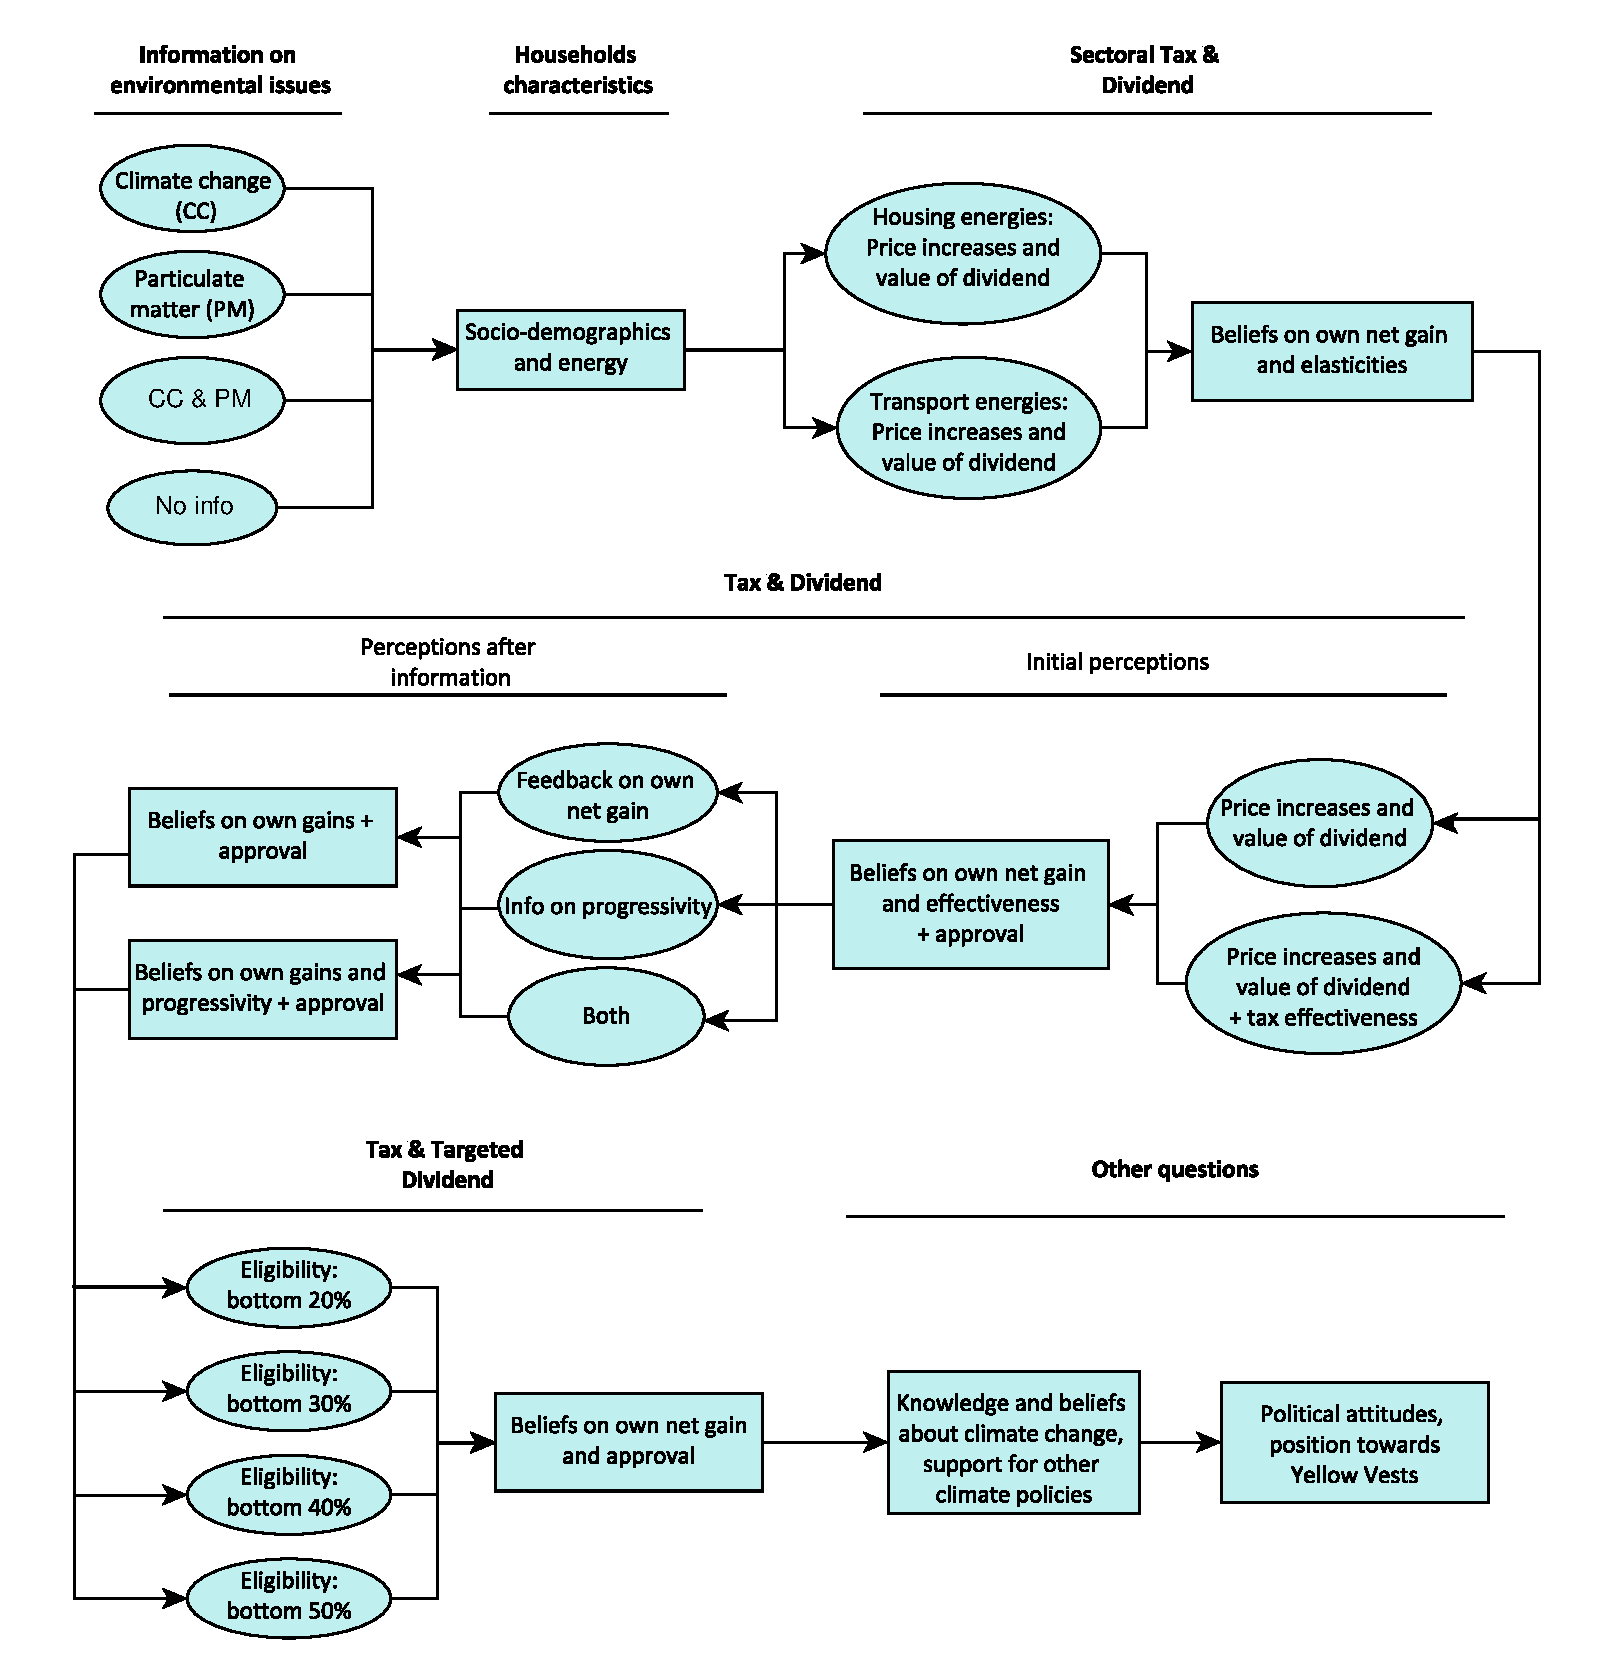
\includegraphics[scale=0.43,left]{Images/diagram_survey.png}

\hyperlink{data_and_policy}{\beamerbutton{Go back}}


% TODO: en appendix

\end{frame}

\begin{frame}{Estimation of increase in housing energy expenditures}\label{estimation_consumption}

{ \scriptsize
\begin{table}[!htbp] \centering 
\caption{Determinants of housing energy expenditures} 
\label{tab:reg_housing} 
\makebox[\textwidth][c]{ \begin{tabular}{@{\extracolsep{5pt}}lccc} 
\\[-1.8ex]\hline 
\hline \\[-1.8ex]
\\[-1.8ex] & \multicolumn{3}{c}{Increase in housing energy expenditures (\euro{}/year)} \\ 
\\[-1.8ex] & (1) & (2) & (3)\\ 
\hline \\[-1.8ex] 
Constant & $-$55.51$^{***}$ &  & $-$0.634  \\ 
& (1.237) &  & (1.489)  \\ 
Housing energy: Gas & 124.6$^{***}$ &  & 1.173 \\ 
& (1.037) &  & (2.323) \\ 
Housing energy: Fuel oil & 221.1$^{***}$ & 129.8$^{***}$ & 130.4$^{***}$ \\ 
& (1.719) & (3.752) &  (4.002) \\ 
Accommodation size (m$^\text{2}$) & 0.652$^{***}$ &  & 0.024 \\ 
& (0.012) &  &  (0.015) \\ 
Accommodation size $\times$ Gas  &  & 1.425$^{***}$ & 1.397$^{***}$ \\ 
&  & (0.007)  & (0.024) \\ 
Accommodation size $\times$ Fuel oil &  & 0.945$^{***}$ & 0.922$^{***}$ \\ 
&  & (0.029)  & (0.032) \\ 
\hline \\[-1.8ex] 
Observations & 26,729 & 26,729 & 26,729 \\ 
R$^{2}$ & 0.545 & 0.716 & 0.599 \\ 
Error rate & 0.166 & 0.155 & 0.155 \\
\hline 
\hline \\[-1.8ex] 
\textit{Note:}  & \multicolumn{3}{r}{$^{*}$p$<$0.1; $^{**}$p$<$0.05; $^{***}$p$<$0.01} \\ 
\end{tabular} 
} \end{table} }

\hyperlink{consumer_survey_data}{\beamerbutton{Go back}}

\end{frame}
\begin{frame}{Prediction's precision} \label{prediction_precision}

\begin{figure}
\includegraphics[width=\columnwidth]{Images/proba_correct_prediction.png}
\caption{Probability that our estimation of net gains correctly predicts the winning category.}
\end{figure}

\hyperlink{consumer_survey_data}{\beamerbutton{Go back}}

\end{frame}


\begin{frame}{Biased perception of net gain}\label{biased_perception_CDF}

    \textcolor{blue}{Objective} vs. \textcolor{red}{subjective} net gains from Tax \& Dividend (in \euro{} per year per c.u.): \hyperlink{biased_perception_PDF}{\beamerbutton{Go back}}
    
    \begin{figure}
      \includegraphics[width=0.4\textwidth]{Images/cdf_carbon_tax_all.png}
      \caption{Net gain. Mean: \textcolor{blue}{- - - -}: case of inelastic expenditures.}
    \end{figure}
    % \begin{columns}[onlytextwidth]
    % \begin{column}{.33\textwidth}
    % \begin{figure}
    %   \includegraphics[width=\textwidth]{Images/cdf_transport_all.png}
    %   \caption{Transport}
    % \end{figure}
    % \end{column}
    % \hfill
    % \begin{column}{.33\textwidth}
    % \begin{figure}
    %   \includegraphics[width=\textwidth]{Images/cdf_housing_all.png}
    %   \caption{Housing}
    % \end{figure}
    % \end{column}
    % \hfill
    % \begin{column}{.33\textwidth}
    % \begin{figure}
    %   \includegraphics[width=\textwidth]{Images/cdf_carbon_tax_all.png}
    %   \caption{Both}
    % \end{figure}
    % \end{column}
    % \end{columns}
    
    \bigskip
    
    
    %\vspace{0.4cm}
    
    Assuming that everyone's fossils consumption is totally inelastic: \vspace{0.1cm}
    \begin{itemize}
        \item 77\% underestimate their gain, 37\% by more than 110\euro{}.  \vspace{0.1cm}
        \item Median gap: 80\euro{}.
    \end{itemize}
    
    
\end{frame}

\begin{frame}{Heterogeneity in bias}

    \vspace{-0.3cm}
    
    {\tiny
    
    \begin{table}[H] \centering 
      \caption{Determinants of a large bias in subjective gains.} 
      \label{tab:bias} 
    \makebox[\textwidth][c]{ \begin{tabular}{@{\extracolsep{5pt}}lccc} 
    \\[-1.8ex]\hline 
    \hline \\[-1.8ex] 
    \\[-1.8ex] & \multicolumn{3}{c}{Large bias (bias $> 110$)} \\ 
    \\[-1.8ex] & \textit{OLS} & \textit{logit} & \textit{OLS} \\ 
    \hline \\[-1.8ex] 
    % Constant & 0.899$^{***}$ &  & 1.032$^{***}$ \\ 
    %  & (0.191) &  & (0.187) \\ 
      Initial tax: PNR (I don't know) &  &  & $-$0.179$^{***}$ \\ 
      &  &  & (0.023) \\ 
      Initial tax: Approves &  &  & \textbf{\textcolor{teal_dark}{$-$0.284$^{***}$}} \\ 
      &  &  & \textbf{\textcolor{teal_dark}{(0.031)}} \\ 
      Sex: Female & 0.036$^{*}$ & 0.030 & 0.042$^{**}$ \\ 
      & (0.020) & (0.020) & (0.019) \\ 
      Ecologist & \textbf{\textcolor{teal_dark}{$-$0.064$^{**}$}} & $-$0.061$^{**}$ & $-$0.025 \\ 
      & \textbf{\textcolor{teal_dark}{(0.026)}} & (0.026) & (0.026) \\ 
      Yellow Vests: PNR & 0.039 & 0.035 & 0.024 \\ 
      & (0.036) & (0.035) & (0.036) \\ 
      Yellow Vests: understands & 0.081$^{***}$ & 0.062$^{***}$ & 0.041$^{*}$ \\ 
      & (0.025) & (0.024) & (0.025) \\ 
      Yellow Vests: supports & 0.108$^{***}$ & 0.103$^{***}$ & 0.051$^{*}$ \\ 
      & (0.026) & (0.025) & (0.026) \\ 
      Yellow Vests: is part & \textbf{\textcolor{teal_dark}{0.202$^{***}$}} & 0.193$^{***}$ & \textbf{\textcolor{teal_dark}{0.147$^{***}$}} \\ 
      &  \textbf{\textcolor{teal_dark}{(0.048)}} & (0.040) & \textbf{\textcolor{teal_dark}{(0.047)}} \\ 
     \hline \\[-1.8ex] 
    Controls: Socio-demo, political leaning & \checkmark & \checkmark & \checkmark \\ 
    Observations & 3,002 & 3,002 & 3,002 \\ 
    R$^{2}$ & 0.061 &  & 0.098 \\ 
    \hline 
    \hline \\[-1.8ex] 
    & \multicolumn{3}{r}{$^{*}$p$<$0.1; $^{**}$p$<$0.05; $^{***}$p$<$0.01} \\ 
    \end{tabular} 
    } \end{table}
    }
    
    \vspace{0.05cm}
    
    $\rightarrow$ The more opposed to the tax, the more biased? Or opposite direction of causality?
    
        \end{frame}
%     \begin{frame}{Tax \& Targeted Dividend: a primer}

% % TODO: merge these two graphs

% \includegraphics[width=0.9\textwidth,left]{Images/RDD_Acceptance_flat_90CI.png}

% % \begin{overprint}
% % \onslide<1>\includegraphics[width=\textwidth,left]{Images/RDD_Acceptance_flat_1.png}
% % \onslide<2>\includegraphics[width=\textwidth,left]{Images/RDD_Acceptance_flat_2.png}
% % \onslide<3>\includegraphics[width=\textwidth,left]{Images/RDD_Acceptance_flat_3.png}
% % \onslide<4>\includegraphics[width=\textwidth,left]{Images/RDD_Acceptance_flat.png}
% % \onslide<5>\includegraphics[width=\textwidth,left]{Images/RDD_Acceptance_flat_90CI.png}
% % \end{overprint}

% \vspace{0.3cm}

% \hyperlink{identification_strategy_si}{\beamergotobutton{Go back}}

%     \end{frame}
%     \begin{frame}{Descriptive statistics on income targets}\label{income_target}


% \medskip
% \hyperlink{identification_strategy_si}{\beamergotobutton{Go back}}
    
%     \end{frame}
    \begin{frame}{First stage self-interest}\label{first_stage_si}

{\tiny
\begin{table}[!htbp] \centering 
  \caption{First stage regressions results for self-interest} 
  \label{first_stage_private_benefits} 
\makebox[\textwidth][c]{ \begin{tabular}{@{\extracolsep{5pt}}lcccc} 
\\[-1.8ex]\hline 
\hline \\[-1.8ex] 
 & \multicolumn{4}{c}{Believes does not lose} \\ 
\cline{2-5} 
\\[-1.8ex] & \multicolumn{2}{c}{Targeted tax ($G^T$)} & \multicolumn{2}{c}{After feedback ($G^F$)} \\ 
 & (1) & (2) & (5) & (6) \\ 
\hline \\[-1.8ex] 
 Transfer to respondent ($T_1$) & 0.268$^{***}$ & 0.227$^{***}$ &  &  \\ 
  & (0.028) & (0.027) &  &  \\ 
  Transfer to spouse ($T_2$) & 0.180$^{***}$ & 0.174$^{***}$ &  &  \\ 
  & (0.031) & (0.030) &  &  \\ 
  $T_1 \times T_2$ & $-$0.190$^{***}$ & $-$0.161$^{***}$ &  &  \\ 
  & (0.038) & (0.037) &  &  \\ 
  Initial tax Acceptance ($A^I$) &  & 0.163$^{***}$ &  & 0.333$^{***}$ \\ 
  &  & (0.033) &  & (0.038) \\ 
  Simulated winner ($\widehat{\Gamma}$) &  &  & 0.217$^{***}$ & 0.210$^{***}$ \\ 
  &  &  & (0.036) & (0.035) \\ 
 \hline \\[-1.8ex] 
Controls: Incomes &  \checkmark &  \checkmark &  &  \checkmark \\ 
Controls: Estimated gain &  &  \checkmark  &  \checkmark &  \checkmark \\ 
Controls: Target of the tax, single &  \checkmark &  \checkmark &   &   \\ 
Controls: Socio-demo, other motives &  &  \checkmark &   &  \checkmark \\ 
Effective F-Statistic (Montiel \& Pflueger, 2013) & 44.093 & 40.834 & 37.966 & 57.866 \\ 
Observations & 3,002 & 3,002 & 1,968 & 1,968 \\ 
R$^{2}$ & 0.082 & 0.177 & 0.131 & 0.319 \\ 
\hline 
\hline \\[-1.8ex] 
& \multicolumn{4}{r}{$^{*}$p$<$0.1; $^{**}$p$<$0.05; $^{***}$p$<$0.01} \\ 
\end{tabular} 
} \end{table} 
}
\medskip
\hyperlink{second_stage_si}{\beamergotobutton{Go back}}

    \end{frame}
    \begin{frame}{First stage environmental effectiveness}\label{first_stage_ee}

{\tiny
\begin{table}[!htbp] \centering 
  \caption{First stage regressions results for environmental effectiveness} 
  \label{first_stage_environmental_effectiveness} 
\makebox[\textwidth][c]{ \begin{tabular}{@{\extracolsep{5pt}}lccc} 
\\[-1.8ex]\hline 
\hline \\[-1.8ex] 
 & \multicolumn{3}{c}{Environmental effectiveness} \\ 
\cline{2-4} 
\\[-1.8ex] & \multicolumn{2}{c}{not ``No''} & ``Yes'' \\ 
 & (1) & (2) & (5,6) \\ 
\hline \\[-1.8ex] 
 Info on Environmental Effectiveness ($Z_{E}$) & 0.062$^{***}$ & 0.043$^{**}$ & 0.059$^{***}$ \\ 
  & (0.017) & (0.017) & (0.014) \\ 
  Info on Climate Change ($Z_{CC}$) & 0.030$^{*}$ & 0.024 & 0.028$^{**}$ \\ 
  & (0.017) & (0.017) & (0.013) \\ 
 \hline \\[-1.8ex] 
Controls: Socio-demo, other motives,  &  \checkmark &  &  \checkmark \\ 
\hspace{1.6cm} incomes, estimated gains  &  & &  \\
Effective F-Statistic (Montiel \& Pflueger, 2013) & 5.866 & 2.523 & 11.145 \\ 
Observations & 3,002 & 3,002 & 3,002 \\ 
R$^{2}$ & 0.121 & 0.003 & 0.123 \\ 
\hline 
\hline \\[-1.8ex] 
& \multicolumn{3}{r}{$^{*}$p$<$0.1; $^{**}$p$<$0.05; $^{***}$p$<$0.01} \\ 
\end{tabular} 
} \end{table} 
}
\medskip
\hyperlink{second_stage_ee}{\beamergotobutton{Go back}}

    \end{frame}
    \begin{frame}{Evidence of motivated reasoning -- robustness heterogeneous priors}\label{rob_mr}

\vspace{-0.2cm}   

\begin{table}[!htbp] \centering 
  \caption{Asymmetric updating of winning category (complementary results).\hyperlink{mr}{\beamergotobutton{Go back}}} 
  \label{tab:robustness_mr2} \vspace{-0.2cm}
\resizebox{0.4\columnwidth}{!}{\begin{tabular}{@{\extracolsep{5pt}}lcc} 
\\[-1.8ex]\hline 
\hline \\[-1.8ex] 
\\[-1.8ex] & \multicolumn{2}{c}{Correct updating ($U$)} \\ 
%\\[-1.8ex] & (1) & (2)\\ 
\hline \\[-1.8ex] 
% Constant & $-$0.146 & $-$0.039 \\ 
 % & (0.178) & (0.179) \\ 
  Winner, before feedback ($\dot{G}$) & 0.646$^{***}$ & 0.551$^{***}$  \\ 
  & (0.080) & (0.083) \\ 
  Initial tax: PNR (I don't know) & 0.163$^{***}$ & 0.179$^{***}$ \\ 
  & (0.031) & (0.032) \\ 
  Initial tax: Approves & 0.158$^{***}$ & \textbf{\textcolor{teal_dark}{0.176$^{***}$}} \\ 
  & (0.046) & \textbf{\textcolor{teal_dark}{(0.046)}} \\ 
  Subjective gain ($g$) &  & \textbf{\textcolor{teal_dark}{0.0004$^{**}$}} \\ 
  &  & \textbf{\textcolor{teal_dark}{(0.0002)}} \\ 
  Subjective gain: unaffected ($g=0$) &  & $-$0.127$^{***}$ \\ 
  &  & (0.033) \\ 
  Bias about gain ($g - \hat{\gamma}$) &  & $-$0.00005 \\ 
  &  & (0.0001) \\ 
  Diploma (1 to 4) & 0.016 & 0.014 \\ 
  & (0.013) & (0.013) \\ 
  Retired & 0.146$^{*}$ & 0.130$^{*}$ \\ 
  & (0.079) & (0.079) \\ 
  Active & 0.175$^{***}$ & 0.166$^{***}$ \\ 
  & (0.054) & (0.054) \\ 
  Student & 0.234$^{***}$ & 0.224$^{***}$ \\ 
  & (0.075) & (0.075) \\ 
  Yellow Vests: PNR & $-$0.043 & $-$0.045 \\ 
  & (0.047) & (0.047) \\ 
  Yellow Vests: understands & $-$0.063$^{*}$ & $-$0.065$^{*}$ \\ 
  & (0.034) & (0.034) \\ 
  Yellow Vests: supports & $-$0.059$^{*}$ & $-$0.063$^{*}$ \\ 
  & (0.036) & (0.036) \\ 
  Yellow Vests: is part & $-$0.137$^{**}$ & \textbf{\textcolor{teal_dark}{$-$0.141$^{**}$}} \\ 
  & (0.062) & \textbf{\textcolor{teal_dark}{(0.061)}} \\ 
 \hline \\[-1.8ex] 
Among invalidated & \checkmark & \checkmark \\ 
Includes controls & \checkmark & \checkmark \\ 
Observations & 1,365 & 1,365 \\ 
R$^{2}$ & 0.133 & 0.144 \\ 
\hline 
\hline \\[-1.8ex] 
& \multicolumn{2}{r}{$^{*}$p$<$0.1; $^{**}$p$<$0.05; $^{***}$p$<$0.01} \\ 
\end{tabular} 
 }
 \end{table}  


    \end{frame}

\begin{frame}{Bias persistence over progressivity}\label{progreg_target}
    It seems we do not convince people at all here ! How come?

\medskip

$\Rightarrow$ Evidences of psychological reactance from biased people (boomerang effect, see Hovland 1953):


{\scriptsize
\begin{table}[!htbp] \centering 
  \caption{Effect of information on perceived progressivity} 
  \label{tab:prog} 
\makebox[\textwidth][c]{ \begin{tabular}{@{\extracolsep{5pt}}lccc} 
\\[-1.8ex]\hline 
\hline \\[-1.8ex] 
\\[-1.8ex] & \multicolumn{3}{c}{Progressivity: not No ($P$)} \\ 
\\[-1.8ex] & (1) & (2) & (3)\\ 
\hline \\[-1.8ex] 
 Constant & 0.419$^{***}$ & 0.435$^{***}$ & 0.386$^{**}$ \\ 
  & (0.022) & (0.033) & (0.186) \\ 
  Information on progressivity ($Z_P$) & $-$0.021 & 0.050 & 0.014 \\ 
  & (0.027) & (0.040) & (0.239) \\ 
  Large bias $(\left|\widehat{\gamma}-g\right|>110)$ &  & $-$0.028 & $-$0.019 \\ 
  &  & (0.045) & (0.045) \\ 
  Interaction $Z_P \times (\left|\widehat{\gamma}-g\right|>110)$ &  & $-$0.130$^{**}$ & $-$0.126$^{**}$ \\ 
  &  & (0.055) & (0.055) \\ 
 \hline \\[-1.8ex] 
Controls: Socio-demo, politics  &  &  & \checkmark  \\ 
Observations & 1,444 & 1,444 & 1,444 \\ 
R$^{2}$ & 0.0004 & 0.018 & 0.100 \\ 
\hline 
\hline \\[-1.8ex] 
& \multicolumn{3}{r}{$^{*}$p$<$0.1; $^{**}$p$<$0.05; $^{***}$p$<$0.01} \\ 
\end{tabular} 
 } \end{table}  
}

\medskip

\hyperlink{progreg_origin}{\beamergotobutton{go back}}

\end{frame}

\begin{frame}{Subjective elasticities}\label{elast_target}
$\rightarrow$ Tempting interpretation: people perceive aggregate consumption as inelastic (Kallbekken \& Sælen, 2011; Carattini et al, 2018)

%\pause

{\scriptsize

\begin{table}[!htbp] \centering 
  \caption{Effect of subjective elasticities on perceived environmental effectiveness} 
  \label{table:elasticities_effectiveness} 
\makebox[\textwidth][c]{ \begin{tabular}{@{\extracolsep{5pt}}lcccc} 
\\[-1.8ex]\hline 
\hline \\[-1.8ex] 
\\[-1.8ex] & \multicolumn{4}{c}{Environmental effectiveness: not `No'} \\ 
\\[-1.8ex] & (1) & (2) & (3) & (4)\\ 
\hline \\[-1.8ex] 
 Price elasticity: Housing & $-$0.062$^{*}$ &  & $-$0.055$^{*}$ &  \\ 
  & (0.032) &  & (0.032) &  \\ 
  Price elasticity: Transports &  & $-$0.056$^{*}$ &  & $-$0.060$^{**}$ \\ 
  &  & (0.030) &  & (0.030) \\ 
 \hline \\[-1.8ex] 
Controls: Socio-demographics, energy &  &  & \checkmark   & \checkmark \\ 
Observations & 1,501 & 1,501 & 1,501 & 1,501 \\ 
R$^{2}$ & 0.003 & 0.002 & 0.089 & 0.090 \\ 
\hline 
\hline \\[-1.8ex] 
\textit{Note:}  & \multicolumn{4}{r}{$^{*}$p$<$0.1; $^{**}$p$<$0.05; $^{***}$p$<$0.01} \\ 
\end{tabular} 
} \end{table} 
}

\medskip

Effect too small to explain the beliefs. 
\medskip

    \hyperlink{elast_origin}{\beamergotobutton{Go back}}
\end{frame}

    \begin{frame}{Asymmetric beliefs' revision}\label{revision_beliefs}

    \hyperlink{bsi}{\beamergotobutton{Go back}}

\vspace{-0.3cm}

{ % \small
\begin{table}[!htbp] \centering 
  \caption{Share of respondents with new beliefs aligned with feedback}
  \label{table:confidence_intervals_beliefs_feedback} 
\resizebox{0.55\columnwidth}{!}{\begin{tabular}{@{\extracolsep{5pt}}lcc} 
\\[-1.8ex]\hline 
\hline \\[-1.8ex] 
 & \multicolumn{2}{c}{\textit{Aligned with feedback}} \\ 
\cline{2-3} 
\\[-1.8ex] & winners & losers \\ \vspace*{0.5cm} & (75.8\%)  & (24.2\%) \\ \hline \\[-1.8ex] 
 Initial belief: win & 78.8\% & 81.5\% \\ 
 (14.0\%) & {\small[73.2\% ; 83.4\%]} & {\small[65.0\% ; 91.3\%]} \\ 
  & & \\ 
 Initial belief: unaffected & 21.6\% & 44.9\% \\ 
 (21.7\%) & {\small[17.6\% ; 26.2\%]} & {\small[33.5\% ; 56.8\%]} \\ 
  & & \\ 
 Initial belief: lose & 12.2\% & 93.9\% \\ 
 (64.3\%) & {\small[10.3\% ; 14.5\%]} & {\small[90.9\% ; 96.0\%]} \\ 
  & & \\[-1.8ex]\hline 
  All & \textcolor{teal_dark}{25.1\%} & \textcolor{teal_dark}{85.7\%} \\ 
 (100\%) & {\small[23.0\% ; 27.3\%]} & {\small[82.2\% ; 88.7\%]} \\ 
 & & \\[-1.8ex]\hline 
\hline \\[-1.8ex]
\end{tabular}}{\footnotesize
\\ \quad \\
\textsc{Note:} The 95\% confidence intervals for binomial probabilities is given in brackets.
}
\end{table}
}

    \end{frame}


\end{document}






% % Trash:

%     \begin{frame}{Consistency with Bayesianism}

% Following Bayes rule, we should theoretically expect respondent $i$ with private information $J_i$ to update its beliefs as follows:

% $$
% \mathbb{P}(G_i^F | \hat{\Gamma}_i, J_i) = \mathbb{P}(G_i | J_i) \frac{
%     \mathbb{P}(\hat{\Gamma}_i | G_i, J_i)
% }{
%     \mathbb{P}(\hat{\Gamma}_i | J_i)
% }
% $$

% \medskip

% \noindent
% with $\mathbb{P}(G_i | J_i)$ its prior probability to win, and $\mathbb{P}(G_i^F | \hat{\Gamma}_i, J_i)$ its posterior after being provided new information. If everyone gives a correct weight to the new information, we should expect:

% $$
% \frac{1}{N_{\hat{\Gamma}}}\sum_{i=1}^{N_{\hat{\Gamma}}} \mathbb{P}(G_i^F = \hat{\Gamma}_i | \hat{\Gamma}_i, J_i) = \frac{5}{6}
% $$

% \medskip
% \pause

% $\Rightarrow$ The null hypothesis of equality with 5/6 is clearly rejected for $\hat{\Gamma} > 0$. Results more contrasted for $\hat{\Gamma} < 0$. How to reconcile this with Bayesian rationality?

% \begin{itemize}
%     \item Respondents think our feedback is biased
%     \item Respondents give too much value to their (biased) private information
% \end{itemize}

% Impossible to disentangle both mechanisms as they both lead to more pessimism.
% % TODO: define notations in first section

% % TODO: change this slide. Stress importance of (1) asymmetric updating, (2) conservatism. Interpret (give possible mechanism, say it reveals pessimism). Link with literature?

%     \end{frame}

